\documentclass[11pt,a4paper]{article}
\usepackage{lmodern}
\usepackage{amssymb,amsmath}
\usepackage{ifxetex,ifluatex}
\usepackage{fixltx2e} % provides \textsubscript
\ifnum 0\ifxetex 1\fi\ifluatex 1\fi=0 % if pdftex
  \usepackage[T1]{fontenc}
  \usepackage[utf8]{inputenc}
\else % if luatex or xelatex
  \ifxetex
    \usepackage{mathspec}
  \else
    \usepackage{fontspec}
  \fi
  \defaultfontfeatures{Ligatures=TeX,Scale=MatchLowercase}
\fi
% use upquote if available, for straight quotes in verbatim environments
\IfFileExists{upquote.sty}{\usepackage{upquote}}{}
% use microtype if available
\IfFileExists{microtype.sty}{%
\usepackage{microtype}
\UseMicrotypeSet[protrusion]{basicmath} % disable protrusion for tt fonts
}{}
\usepackage[top=3cm,left=3cm,right=3cm]{geometry}
\usepackage{hyperref}
\hypersetup{unicode=true,
            pdftitle={Disease Modeling},
            pdfborder={0 0 0},
            breaklinks=true}
\urlstyle{same}  % don't use monospace font for urls
\usepackage{longtable,booktabs}
\usepackage{graphicx,grffile}
\makeatletter
\def\maxwidth{\ifdim\Gin@nat@width>\linewidth\linewidth\else\Gin@nat@width\fi}
\def\maxheight{\ifdim\Gin@nat@height>\textheight\textheight\else\Gin@nat@height\fi}
\makeatother
% Scale images if necessary, so that they will not overflow the page
% margins by default, and it is still possible to overwrite the defaults
% using explicit options in \includegraphics[width, height, ...]{}
\setkeys{Gin}{width=\maxwidth,height=\maxheight,keepaspectratio}
\IfFileExists{parskip.sty}{%
\usepackage{parskip}
}{% else
\setlength{\parindent}{0pt}
\setlength{\parskip}{6pt plus 2pt minus 1pt}
}
\setlength{\emergencystretch}{3em}  % prevent overfull lines
\providecommand{\tightlist}{%
  \setlength{\itemsep}{0pt}\setlength{\parskip}{0pt}}
\setcounter{secnumdepth}{5}
% Redefines (sub)paragraphs to behave more like sections
\ifx\paragraph\undefined\else
\let\oldparagraph\paragraph
\renewcommand{\paragraph}[1]{\oldparagraph{#1}\mbox{}}
\fi
\ifx\subparagraph\undefined\else
\let\oldsubparagraph\subparagraph
\renewcommand{\subparagraph}[1]{\oldsubparagraph{#1}\mbox{}}
\fi

%%% Use protect on footnotes to avoid problems with footnotes in titles
\let\rmarkdownfootnote\footnote%
\def\footnote{\protect\rmarkdownfootnote}

%%% Change title format to be more compact
\usepackage{titling}

% Create subtitle command for use in maketitle
\providecommand{\subtitle}[1]{
  \posttitle{
    \begin{center}\large#1\end{center}
    }
}

\setlength{\droptitle}{-2em}

  \title{Disease Modeling}
    \pretitle{\vspace{\droptitle}\centering\huge}
  \posttitle{\par}
    \author{}
    \preauthor{}\postauthor{}
    \date{}
    \predate{}\postdate{}
  
\usepackage{multirow}
\usepackage{multicol}
\usepackage{booktabs}
\usepackage{xcolor}
\numberwithin{equation}{section}
\usepackage{dcolumn}
\usepackage{rotating}
\usepackage{caption}
\usepackage{amsfonts}
\captionsetup{width=4.5in}
\usepackage{mathtools}

\begin{document}
\maketitle

\newcommand{\dw}[1]{{\color{red}{#1}}}
\newcommand{\del}[1]{{\color{blue}{}}}

\hypertarget{intro}{%
\section{Intro}\label{intro}}

In this thesis we perform inference on an extension of a model presented
by Held et al. (\protect\hyperlink{ref-held_two-component_2006}{2006})
for infectious disease surveillance data. Their method models infectious
disease incidence (i.e., new cases) as a branching Poisson process with
a cyclical endemic parameter. The cyclical endemic parameter models
``seasonality'' (e.g.~seasonal flu patterns) while the Poisson branching
process allows for ``outbreaks'' (e.g.~swine flu, H1N1). Their method
models a single time series of count data from a specific location or
region. We extend the model to multiple time series of count data that
are spatially related.

The dataset of interest contains data from 412 administrative districts
in Germany. Each district has surveillance data which contains the
weekly case counts of severe gastroenteritis or stomach flu. The data
spans May 2 and July 26 2011 when a strain of \emph{Escherichia coli}
(\emph{E. coli}) caused an outbreak of severe illness in Germany. Over
3,950 people were affected compared with the typically seen
\textasciitilde{}200 cases a year typically seen. Many developed severe
complications and over 50 people died tk fix citation (\emph{EHEC O104}
\protect\hyperlink{ref-noauthor_ehec_2011}{2011} , pp.~2-3, 11).

We to extend the model to incorporate a graph that epresents a
transmission network between the different spatial regions (e.g., the
administration district) and allow dependencies between count data in
those regions. The end goal will be to be able to estimate covariates
that affect the probability of transmission between regions (e.g., the
shipping network that transmitted the \emph{E. coli} contaminated food).

Statistical methods to model infectious disease data typically use
mechanistic models that is models that use expert knowledge of the
underyling process (Pawitan
\protect\hyperlink{ref-pawitan_all_2001}{2001}, ch.~1). One such model
is the Susceptible-(Exposed)-Infectious-Recovery (SIR/SEIR) (Keeling and
Rohani \protect\hyperlink{ref-keeling_modeling_2008}{2008} , pp.~41-43)
model and other variants. In the SEIR model, the entire closed
population of individuals is in one of the four states. susceptible
individuals can become exposed when in contact with an infectious
invidual, exposed individuals will eventually become infectious and
infectious individuals will eventually be recovered and cannot be
re-exposed or infect susceptibles (e.g.~by immunity). Given partial data
on the susceptible, exposed, infectious and removed times parameters
surrounding the epidemic of interest can be estimated. For example, in
Groendyke et al.
(\protect\hyperlink{ref-groendyke_bayesian_2011}{2011}), the time spent
in each state is modeled with a Gamma random variables and the
parameters of the random variables can be estimated from the data. Other
parameters of interest such as the intial infected can also be
estimated. They also estimate contact network between individuals,
covariates affecting the formation of the contact network and a
corresponding transmission tree. While effective, this sort of
mechanistic model requires data at a granularity not typical of
surveillance data, (such as information on the susceptibles) and often
contains other problems such as underreporting (Diggle et al.
\protect\hyperlink{ref-diggle_-line_2003}{2003} , pp.~233-266)

\hypertarget{intro-to-two-component-model}{%
\section{Intro to Two-Component
Model}\label{intro-to-two-component-model}}

Held et al. (\protect\hyperlink{ref-held_two-component_2006}{2006})
presents a stochastic model for the statistical analysis of infectious
disease counts that serves as the basis of the theextended graph model.

The two components of the model are a simple Poisson branching process
with autoregressive parameter \(\lambda\) and a seasonal component fit
with a Fourier series. These components are described as the
``epidemic'' and ``endemic'' components respectively. Additionally, the
two-component model allows for \(\lambda\) to change over time
representing changing infectivity.

A branching process is a model that is used to model the evolution
(Grimmett and Stirzaker
\protect\hyperlink{ref-grimmett_probability_2004}{2004} , pp.~171-175,
243-255) of population over time. Suppose there's currently one parent
alive (cf., one person infectious). Then in a branching process, this
individual would give birth to a random number of offspring (cf., newly
infected) and then immediately die. Then at the next step, each of those
offspring become parents who individually give birth to a random number
of offspring. If the random number of offspring comes from a Poisson
distribution, then the process is known as a Poisson branching process.
its in this sense that \(\lambda\) is an autoregressive parameter since
it describes the relationship between the individuals in the previous
time step to the current one. In thise case we assume that the
\(\lambda\) value is constant across individuals and over time
(e.g.~\(\lambda\) is some biological reproduction rate). In the case of
the Two-Component model, is fixed for individuals at a given time, but
is allowed to vary over time. This allows the model to capture the
dynamics of disease outbreaks.

\hypertarget{two-component-model-notation}{%
\subsection{Two-Component Model
Notation}\label{two-component-model-notation}}

Let \(Z = (Z_0, Z_1, ..., Z_n)\) be the incidence at each time step
\(t\) and let each \(Z_t= Y_t + X_t, t\in \{1,\dots, n\}\). The model is
then specified through \(Z_t | Z_{t-1}\).

\hypertarget{epidemic-component}{%
\subsection{Epidemic Component}\label{epidemic-component}}

The epidemic component is given by

\[Y_t|Z_{t-1} \sim\text{Pois}(\lambda_tZ_{t-1}),\]

where \(\lambda_t\) is the time varing infectivity parameter and
\(Z_{t-1}\) is the the infected count in the previous time step.

We can think of \(\lambda_t\) as the infectivity of the disease at time
\(t\) with an infected person causing new infections as
\(\text{Pois}(\lambda_t)\). Since each infected at time \(Z_{t-1}\)
generates new infected i.i.d \(\text{Pois}(\lambda_t)\), then \(Z_t\) is
the sum of those random variables \del{which itself is Poisson;}
\(\sum_1^{Z_{n-1}}\text{Pois}(\lambda_t) =\text{Pois}(\lambda_tZ_{n-1})\).

In this model, the \(\lambda_t\) is allowed to vary over time. We
restrict \(\lambda\) to be piecewise constant with \(K\) change points
at locations \(\theta_1 < \cdots < \theta_K\) with
\(\theta \in \{1,...,n-1\}\). If \(K = 0\) there is no change point and
the \(\lambda\) parameter is constant throughout.

\hypertarget{tk-add-references-below}{%
\subsection{TK add references below}\label{tk-add-references-below}}

If we only consider the process \(Z_t = Y_t\), when \(\lambda > 1\) an
outbreak occurs (Held et al.
\protect\hyperlink{ref-held_two-component_2006}{2006}). When
\(\lambda < 1\) then the process ``goes extinct'' or reaches and remains
at 0 with probability 1 (Grimmett and Stirzaker
\protect\hyperlink{ref-grimmett_probability_2004}{2004} , pp.~245). Once
the process reaches a point where \(Z_t = 0\), it remains there as there
are no more infected to create new infected at the next time step. When
\(\lambda_t > 1\) an ``outbreak'' occurs shown as the spike in the graph
between. When \(\lambda_t < 1\) the outbreak ends.

Allowing \(\lambda_t\) to vary captures many scenarios, for example a
particulary infectious strain of the flu could cause \(\lambda_t\) to
increase above 1 and cause an outbreak. Later, better or new vaccines
and quarantine procedures can cause the overall infectivity to decrease
below 1.

\hypertarget{endemic-component}{%
\subsection{Endemic Component}\label{endemic-component}}

The endemic component in the model plays two roles. It allows capture of
cyclical behaviors in disease counts (e.g.~seasonal flu) and it also
prevents the branching process from going extinct. The endemic count is
modeled as

\[X_t \sim \text{Pois}(\nu_t)\]
\[\log{\nu_t} = \gamma_0 + \sum_{l = 1}^L (\gamma_{2l-1}\sin(\rho l t)+\gamma_{2l}cos(\rho l t)).\]

That is, \(\log{\nu_t}\) is \del{fit with} a Fourier series which can
approximate any function arbitrarily closely. Following, Held et al.
(\protect\hyperlink{ref-held_two-component_2006}{2006}) the series is
computed with \(L = 1\) since it was determined higher order frequencies
were insignificant. That is the truncated series is still flexible
enough to model cyclical patterns seen in disease counts.

The parameter can then be fit with a linear regression \dw{what relevance does mention of linear regression have here?}
\(\log{\nu_t} = s_t\gamma^T\)
where \dw{don't use angle brackets}
\(s_t = \langle 1, sin(\rho l t), \gamma_{2l}cos(\rho l t) \rangle\).

\begin{figure}
\centering
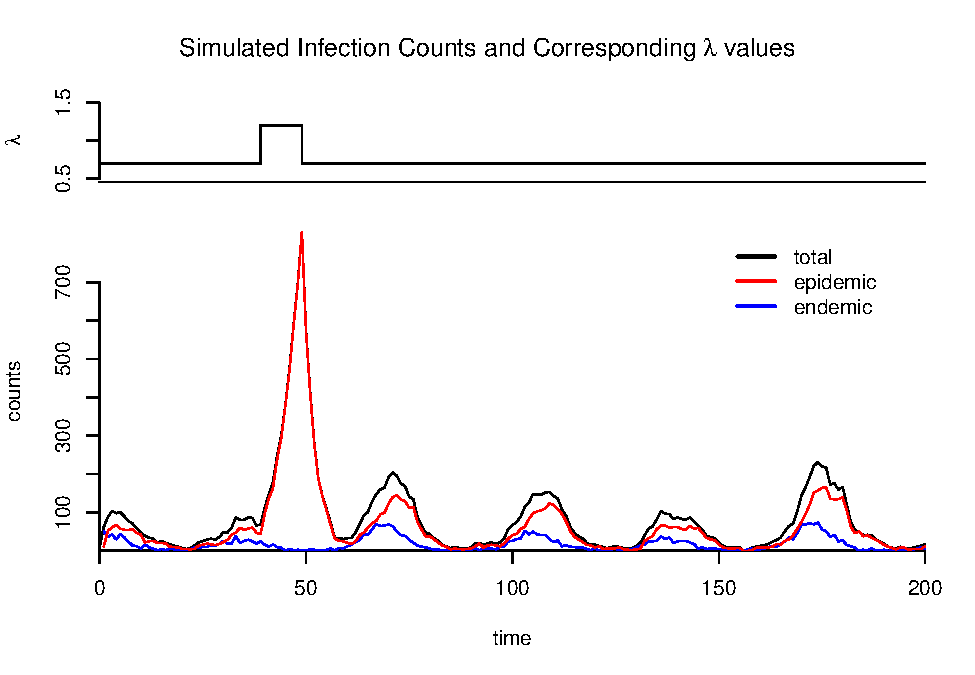
\includegraphics{thesis_draft_files/figure-latex/simulation figure-1.pdf}
\caption{\label{fig:figs}plotting example}
\end{figure}

\hypertarget{likelihood}{%
\subsection{Likelihood}\label{likelihood}}

The probability of the full time series \(Z\) given the initial starting
count \(Z_0\) can be factored as a product of the probabilities of each
\(Z_t\) given the previous count \(Z_{t-1}\),

\[P(Z|Z_0,\theta, K, \lambda^{(1)}, \dots, \lambda^{(K+1)}, \gamma_0, \gamma_1, \gamma_2 ) = \prod_{t=1}^b P(Z_t|Z_t{-1}, \theta, K, \lambda^{(1)}, \dots, \lambda^{(K+1)}, \gamma_0, \gamma_1, \gamma_2),\]
where \(Z_t\) is distributed as sum of the Poisson endemic and epidemic
components,
\[Z_t|Z_{t-1}, \theta, K, \lambda^{(1)}, \dots, \lambda^{(K+1)}, \gamma_0, \gamma_1, \gamma_2 \sim\text{Pois}(\nu_t + \lambda_tZ_{t-1}),\]
\del{where}the endemic component \(\nu_t\) is described as \del{,}
\[\log{\nu_t} = \gamma_0 +  \gamma_{1}\sin(\rho l t)+\gamma_{2}\cos(\rho l t),\]
and \(\lambda_t\) piecewise function is described by
\[ \lambda_t =  \begin{cases} \lambda^{(1)}, & t < \theta_0 \\
\lambda^{(k)}, & \theta_{k} \leq t < \theta_{(k-1)} \\
\lambda^{(K+1)}, & t \geq \theta_K \end{cases}.\]

\hypertarget{multiple-locations-connected-by-a-graph}{%
\section{Multiple locations connected by a
graph}\label{multiple-locations-connected-by-a-graph}}

We would like to extend our data from a univariate time series of counts
\(Z_t\) to a multiple time series of counts \(Z_{i,t}\) where \(i\) now
indexes separate time series. In this case we will say the \(i\) indexes
individual ``cities'' so \(Z_i\) represents the \dw{use incidence here and where appropriate throughout, not infectious disease/epidemic disease counts - and note epidemic means quite a different thing from infectious} infectious disease
counts in city \(i\). Now, a city \(i\)'s epidemic disease count at time
\(t\) is modelled as a function of both its counts \(Z_{i,t-1}\) and
possibly other cites' counts as well.

This dependence between cities is represented by a fixed graph \(G\)
where \(N_v\), the number of vertices in graph is fixed and equal to the
number of cities. An (undirected) edge \(\{i,j\}\) connects vertices
\(i\) and \(j\) if the counts in city \(i\) influences the counts in
city \(j\) and vice versa. We call \(V = \{1,\dots,N_v \}\) the vertex
set of the graph where \(N_v\) is the number of cities/individual time
series of disease counts, and \(E(G)\) is a set of unordered pairs of
vertices \(\{i,j\}\) where \(i,j \in V\) and \(i \neq j\) that describes
the edges present in graph \(G\). We represent the edge \(\{i,j\}\) as
\(e_{ij}\) and the indicator \(1[e_{ij}\dw{]}=1\del{]}\) if \(\{i,j\} \in E(G)\) and
0 otherwise.

\begin{figure}
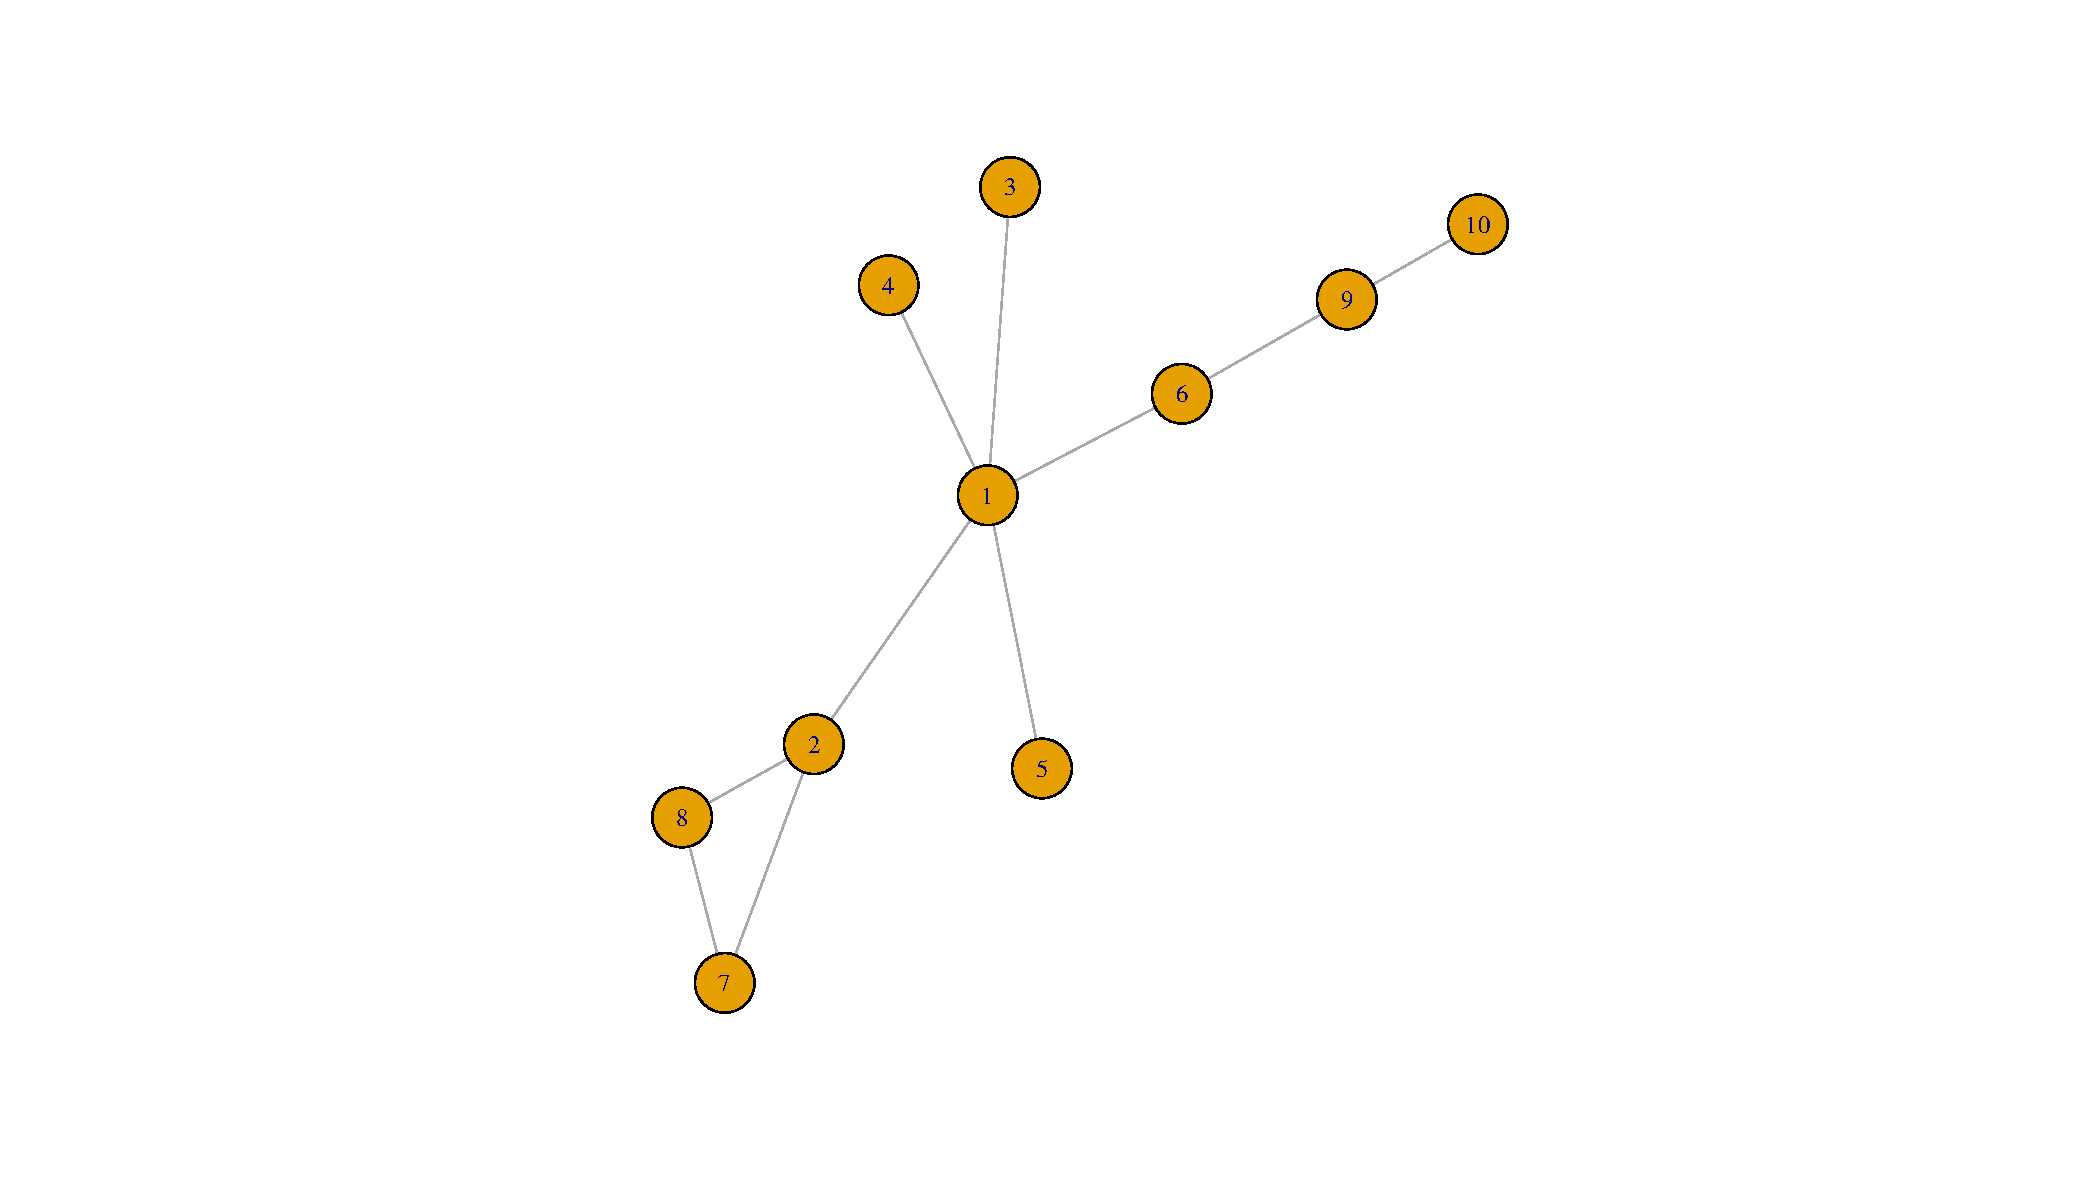
\includegraphics[trim={1 2cm 0 2cm},clip]{thesis_draft_files/figure-latex/unnamed-chunk-1-1} \caption{\label{fig:graph example} A graph configuration. The vertices $i \in \{1,\dots, 10\}$ represent cities each with their own disease counts $Z_{i,t}$. The edges between the graph represent whether the counts between the cities can affect each other. In this example city 1's disease counts at time $t$ are influenced by both its own counts and cities 2, 4, 5 and 6's (i.e., every city connected to it) disease counts. City 10's disease counts are only its own and city 9's.}\label{fig:unnamed-chunk-1}
\end{figure}

We then model the disease count of city \(i\) at time \(t\) as a
function of \(Z_{i,t-1}\) (as before, its own counts at time \(t-1\)) as
well all the counts of the cities \(j\) it is connected to,
\(Z_{j,t-1}\). Then the counts at city \(i\) at time \(t\) are modeled
as \(Z_t|Z_{t-1}, G = X_{i, t} + Y_{i,t}|G\) where \dw{punctuation below}
\[X_{i,t}: \text{infected count in city } i \text{ at time step } t \text{, due to endemic factors}   \]
\[Y_{i,t}|G : \text{infected count in city } i \text{ at time step } t \text{, due to epidemic factors}\]
\[Z_{i,t}|G = X_{i,t} + Y_{i,t}|G: \text{infected count in city } i \text{ at time step } t\]
As before we have the epidemic component as
\(X_{i,t} \sim\text{Pois}(\nu_t)\). For the epidemic component we now
include the additional counts from connected cities as

\[Y_{i,t}|G \sim ~ \text{Pois}\big(\lambda_t\sum_{j\neq i}^{N_v}Z_{j,t-1}1[e_{ij}=1]+ \lambda_tZ_{i,t-1}\big)|G, \]
where \(\lambda_t\sum_{j\neq i}^{N_v}Z_{j,t}1[e_{ij}=1]\) are the counts
from cities connected to city \(i\).

That is, the epidemic component for city \(i\) is the sum of all counts
in every city \(j\) connected to \(i\) in addition to the counts in city
\(i\).

\hypertarget{migration}{%
\subsection{Migration}\label{migration}}

One issue with this model is that connecting two isolated cities
essentially doubles the infectivity parameter, since we include the
counts from both cities. In this formulation a connection between two
cities is equivalent to treating them \dw{as} a single city. To make the model
more realistic, a migration parameter \(m \in (0,1)\) is introduced so

\[Y_{i,t}|G \sim ~ \text{Pois}\big(m\lambda_t\sum_{j\neq i}^{N_v}Z_{j,t-1}1[e_{ij}=1]+ \lambda_tZ_{i,t-1}\big)|G.\]

The migration parameter \(m\) is then the fraction of infected in city
\(j\) that can cause infections in city \(i\), where \(m = 1\) is
equivalent to the previous model and all infected in city \(j\) are
counted and \(m = 0\) is no infected are counted and is equivalent to
the cities \(i,j\) not being connected in graph \(G\) (i.e,
\(e_{ij} \notin G\))

\hypertarget{bayesian-inference}{%
\section{Bayesian Inference}\label{bayesian-inference}}

In Bayesian analysis, we aim to estimate the posterior distribution of
the parameters which we can calculate via Bayes' theorem:
\[ P(\theta|D) = \frac{P(D|\theta)P(\theta)}{P(D)}.\] \(P(\theta|D)\) is
the posterior distribution of the parameters, \(\theta\), given the data
\(D\). \(P(D|\theta)\) is the likelihood of the data \(D\) given the
parameter value \(\theta\) \dw{usually talk about likelihood of parameter}. \(P(\theta)\) is the prior distribution of
\(\theta\) and represents the belief that the parameters will take
certain values \dw{before seeing the data}. If we have little prior information about a parameter,
we try to choose an uninformative prior to reflect that ignorance\dw{.}
\(P(D)\) is the probability of the data marginalized over the parameter
space. One issue is the computation of \(P(\text{D})\) which is given by
\(\int P(\text{D}|\theta)P(\theta)\) over the entire parameter space.
With many parameters this integral it typically analytically
intractable. To handle this Markov chain Monte-Carlo methods are used
which we discuss in section (\#methods \dw{fix reference}).

We now specify the priors of the Two-Component and graph portions of the
model.

\hypertarget{priors-for-lambda-gamma-k-and-vectheta}{%
\subsection{\texorpdfstring{Priors for \(\lambda\), \(\gamma\), \(K\)
and
\(\vec{\theta}\)}{Priors for \textbackslash{}lambda, \textbackslash{}gamma, K and \textbackslash{}vec\{\textbackslash{}theta\}}}\label{priors-for-lambda-gamma-k-and-vectheta}}

The prior distribution for the \(\gamma\) parameters is Normal with
variance \(\sigma^2 = 3^2\) to describe an uninformative prior:

\[\gamma_i \sim N(0, 3I_3), i \in \{0,1,2\}.\]

Since the \(\lambda\) values parameterize a Poisson distribution we set
the prior to be Gamma(1, 1), its conjugate distribution. If Gamma is
interpreted as the sum of exponentials, then the shape = 1, rate = 1
parameterization represents seeing a single occurence in 1 unit of time
and also represents an uninformative prior.

\[ \lambda^{(k)} \sim Gamma(1, 1),\ k \in \{1, \dots, K + 1\}.\]

The number of change points \(K\) takes values in \(\{1,\dots,N\}\)
where \(N\) is the total number of time points of counts collected. In
the Held et al. (\protect\hyperlink{ref-held_two-component_2006}{2006})
paper the number of change points is uniformly distributed
\(P(K = k) = 1/N\) representing uncertainty in the number of change
points. This is changed to \[K \sim \text{Pois}(2)\] representing that
idea that the disease count data is already of interest due to a
potential change in the infectivity of the disease.
\(K \sim\text{Pois}(2)\) places the highest mass on \(K = 2\) change
points which can capture a spike in disease counts (as seen in the
simulated data) before returning to a baseline endemic rate. It also
places mass on \(K = 1\) (e.g.~capturing a long term decrease in
infectivity due to intervention) and \(K = 3\) change points. It also
acts as a regularizer to help reduce overfitting the count time series
where each time point is given a unique \(\lambda_t\) value.

The probability of a specific location for a change point given the
number of change points is uniformly distributed among all the possible
change points, \[P(\theta|K=k) = \binom{N}{k}^{-1}.\] Then the
unnormallized posterior is then the product of the likelihood and the
priors, \dw{delete *'s in below}
\[ P(\theta, K, \lambda^{(1)}, \dots, \lambda^{(K+1)}, \gamma_0, \gamma_1, \gamma_2|Z)  \propto \]
\[\prod_{t=1}^N P(Z_t|Z_{t-1},\theta, K, \lambda^{(1)}, \dots, \lambda^{(K+1)}, \gamma_0, \gamma_1, \gamma_2)*P(\theta|K)*P(K)*P(\prod_{k=1}^{K+1}\lambda^{(k)} )*P(\prod_{i=0}^2 \gamma_i)  .\]

\hypertarget{graph-prior}{%
\subsection{Graph Prior}\label{graph-prior}}

We model the graph \(G\) modeled as an Erdos-Renyi random graph. An
Erdos-Renyi random graph has a fixed vertex set
\(V(G) = \{1, \dots, N_v\}\) and is parameterized by \(p \in (0,1)\) \dw{should be closed interval}.
Then an edge \(e_{ij}\) is in the edge set \(E(G)\) with probability
\(p\) independent of every other edge. That is an ER graph
\(G \sim ER(p)\) and the likelihood of a graph \(G\) given probability
\(p\) on an edge is
\[\begin{aligned} G|p & = \prod_{i,j \in V(G),i \neq j} p^{1[e_{ij}=1]}(1-p)^{1-1[e_{ij}=1]} 
\\ & = p^{N_e}(1-p)^{\binom{N_v}{2}-N_e} \end{aligned}\] where \(N_e\)
is the number of edges.

We then place a prior on \(p\) as \(p \sim Unif(0,1)\) representing lack
of knowledge of the sparseness of the graph. Now computing the marginal
probability of a graph we find \dw{pretty much can get rid of * everywhere unless it is confusing without. And use $\left(\mbox{ and }\right)$ to get bracket sizes right --- oh I see the problem appears to be with binom. maybe redefine that.}
\[ \begin{aligned} P(G)  & = \int_0^1  P(G,p)dp   = \int_0^1 P(G|p)*P(p)dp \\ 
&= \int_0^1 p^{N_e}(1-p)^{\binom{N_v}{2}-N_e}*1*dp = \frac{1}{(\binom{N_v}{2}+1)* \binom{\binom{N_v}{2}}{N_e} }  \end{aligned}\]

That is the probability of graph is proportional to the number of edges
\(|N_e|\) in the graph. In essence the probability of the number of
edges in the graph is uniform with \(P(N_e) = 1/\binom{N_v}{2}\).
However a graph with 2 edges compared with a graph with 1 edge is

\[\begin{aligned}\frac{ P(G_{N_e = 2})}{P(G_{N_e = 1})}  &=  \frac{1/(\binom{N_v}{2}+1)\binom{N_v}{2}}{1/(\binom{N_v}{2}+1)\binom{N_v}{1}} \\& = \frac{\binom{N_v}{1}}{\binom{N_v}{2}}  \\& = \frac{N_v-1}{2},\end{aligned}\]

more likely \dw{this calculation is wrong, you have it upside down -- for large $N_v$ there are far fewer 1 edge graphs than 2 edge ones so each 1 edge one should have a higher prob. so get rid of yr adjustment below}  . Then graphs with \(N_e = \binom{N_v}{2}/2\) are more likely
compared to all graphs with \(|N_e| \in (0, N_v)\) and empty and
complete graphs have the highest probability overall. We instead would
like the probability of a graph to be uniform amongst all possible
graphs. To do so we set a prior on the number of edges so that
\(P(G_{N_e}) = \binom{\binom{N_v}{2}}{N_e}\) .  It may be desirable to
place a \(Beta\) prior in \(p\) with higher mass on lower probabilities \dw{yes, we typically have some idea of the value of $p$}

\hypertarget{posterior}{%
\subsection{Posterior}\label{posterior}}

To summarize posterior is proportional to the product of the likelihood,
graph and non-graph priors

\[ P(\vec{\theta}, K, \lambda^{(1)}, \dots, \lambda^{(K+1)}, \gamma_0, \gamma_1, \gamma_2, G,p|Z)  \propto \]
\[\begin{aligned}\prod_{i=1}^{N_v}\prod_{t=1}^N P(Z_{i,t}|Z_{t-1},\theta, K, \lambda^{(1)}, \dots, \lambda^{(K+1)}, \gamma_0, \gamma_1, \gamma_2,G,p)*\\P(\theta|K)P(K)P(\prod_{k=1}^{K+1}\lambda^{(k)} )P(\prod_{i=0}^2 \gamma_i)P(G|p)P(p), \end{aligned} \]

where \(\vec{\theta}\) is a \(K\) dimensional vector of locations of
change points (and takes values in \(\{1,\dots,N\}\) where \(n\) is end
of the time series), \(\lambda^{(1)}, \dots, \lambda^{(K+1)}\)
parameterize the epidemic component at the corresponding change points,
\(\gamma_0, \gamma_1, \gamma_2\) parameterize the Fourier series that
drives the endemic component, \(G\) is Erdos-Renyi (ER) random graph
that represents the dependencies between cities and \(p \in (0,1)\)
parameterizes the ER graphs and is the probability of an edge being in
the graph.

\hypertarget{metropolis-hastings-algorithm}{%
\subsection{Metropolis-Hastings
Algorithm}\label{metropolis-hastings-algorithm}}

To approximate the posterior, we draw samples from it using the
Metropolis-Hastings algorithm (and its variant, the
Metropolis-Hastings-Green algorithm). The algorithm begins with an
Markov chain with some arbitrary transition probabilities \(q\), whose
state space is the parameter space of the model, \(\theta\) \dw{not a great explanation, you never have a chain with arbitrary transition probabilities. describe it an algorithm that produces a chain with the posterior distributin as its stationary distribution then just given the algorithm}. After
initializing the Markov chain in some initial state \(\theta_0\), the
algorithm modifies the transition probabilities in such a way that the
new transition probabilities has a stationary distribution that is the
target posterior. That is the Markov chain will eventually enter states
in proportion to the posterior distribution.

The algorithm is as follows:

\begin{enumerate}
\def\labelenumi{\arabic{enumi}.}
\item
  Initialize the Markov chain at some state \(\theta_0\)
\item
  From the current state \(\theta\) at time \(n\) propose a new state
  \(j\) according to \(q\). The probability of proposing a transition
  \(\theta \rightarrow \theta^*\) is \(q(\theta^*|\theta)\)
\item
  Compute the acceptance probability
  \[\alpha(\theta^*|\theta) = \min\{1, \frac{P(D|\theta^*)P(\theta^*)}{P(D|\theta)P(\theta)}\frac{q(\theta|\theta^*)}{q(\theta^*|\theta)} \}\]
\item
  Generate \(U \sim Unif(0,1)\)
\item
  If \(U < \alpha(\theta|\theta^*)\) then accept the move and the
  parameter value at time \(n+1\) is \(\theta_{n+1} = \theta^*\). If
  \(U \geq \alpha(\theta|\theta^*)\) reject the move. Then the chain
  remains in the same state at time \(n+1\) and
  \(\theta_{n+1} = \theta\).
\item
  Repeat steps 1-5 for a large number of iterations.
\end{enumerate}

The fraction \(\frac{q(\theta^*|\theta)}{q(\theta|\theta^*)}\) is known
as the Hastings ratio and is a function of the proposal distribution. It
is typically chosen to be symmetric \dw{no its not --- the hastings algoeithm  (Hastings 1970) extended the metropolis et al algorithm which always has this ratio as 1 to work for arbitrary $q$} , if it so that the ratio is always 1. Then
the transition probability is ratio of the posterior distributions whose
denominators, \(P(D)\), cancels leaving
\(\frac{P(D|\theta^*)P(\theta^*)}{P(D|\theta)P(\theta)}\). The proposal
ratio becomes important in asymmetric proposal distributions which
occurs in some of the graph proposals below. For example if two
parameter \(\theta, \theta^*\) values are equally likely,
\(P(\theta^*|D) = P(\theta|D)\) then the Markov chain should enter those
states with the same frequency. However if the proposal distribution
proposes entering \(\theta^*\) twice as frequently as \(\theta^*\), then
without the Hastings ratio there would be twice the frequency of
\(\theta^*\).

A similar issue is also seen when jumping between parameter spaces. To
handle this the Metropolis-Hastings-Green algorithm is introduced which
adds an additional Jacobian term \(|J|\) to handle the change in
dimension. This is described further below.

\hypertarget{model-checking}{%
\subsection{Model Checking}\label{model-checking}}
\dw{move this to after section 6 - it is part of the results }
An important step in all statistical modelling is checking the model.

\hypertarget{prior-checks}{%
\subsubsection{Prior Checks}\label{prior-checks}}

The priors can be checked by setting likelihood to 1. Then the posterior
is only a function of the priors

\[\begin{aligned} P(\theta|D) & \propto P(D|\theta)P(\theta) \\ & \propto 1*P(\theta)  \end{aligned} \]
that is the samples returned by the MCMC should be drawn from the prior
distribution. This helps shows that the prior distributions are properly
implemented in the model as well as show potentially unintended
assumptions about the priors.

Other prior analysis include prior sensitivity analysis where the effect
of different priors on the posterior distribution are examined. This is
less important when the datasets are large sense the likelihood portion
generally dominates the posterior calculation.

\hypertarget{well-calibrated}{%
\subsubsection{Well-Calibrated}\label{well-calibrated}}

A goal of frequentist statistical inference is to obtain confidence
intervals (CI), where a 95\% CI for a parameter would capture the true
parameter in 95\% of replications.

A credible interval plays a similar role in Bayesian inference. We would
like a 95\% credible interval for a parameter to capture the ``true''
parameter value 95\% of the time. If this is the case, then the model is
considered ``well-calibrated''. To do this for Bayesian models, we draw
samples of the estimated parameters from their prior distributions
\(\theta_{sample_1} \sim P(\theta)\) and then using the sampled
parameters we simulate data according to the likelihood function
\(D_{1} \sim P(D|\theta_{sample_1})\). The model is then used to compute
95\% credible intervals as if it were real data. This process is
repeated for
\((\theta_{sample_2}, D_2), \dots, (\theta_{sample_N}, D_N)\) and their
corresponding credible intervals are collected. We can then compare to
see if the 95\% credible intervals from the \(N\) parameter samples,
covers the true sampled parameter 95\% of the time (Carpenter
\protect\hyperlink{ref-carpenter_bayesian_2017}{2017}; Cook et al.
\protect\hyperlink{ref-cook_validation_2006}{2006}).

\hypertarget{posterior-predictive-checking}{%
\subsubsection{Posterior Predictive
Checking}\label{posterior-predictive-checking}}

If the model is a good fit for the data, then simulating data by
sampling according the posterior distribution, should result in
simulated data that looks similar to the true data. If this is not the
case, the model potentially inadequate for capturing important features
of the data. This can be done in a qualitative manner where obviously
poor models can be investigated (Gelman et al.
\protect\hyperlink{ref-gelman_bayesian_2013}{2013},pp. 141--159;
Kruschke \protect\hyperlink{ref-kruschke_doing_2014}{2014},pp. 130--131)

\hypertarget{methods}{%
\section{Methods/ Implementation}\label{methods}}

Here I describe the Metropolis Hastings algorithms used to draw samples
from the posterior distributions of the parameters of interest. The
algorithms are implemented in base R (R Core Team
\protect\hyperlink{ref-r_core_team_r_2019}{2019}) with some elements of
the likelihood computation implemented in Rcpp (Eddelbuettel and
François \protect\hyperlink{ref-eddelbuettel_rcpp_2011}{2011}). The
operators generate and evaluate proposals. Each operator is a R function
that accepts a list of parameters that represent the current state of
the Markov chain, then proposes an new state for a given parameter (or
set of parameters). The function then calculates the log acceptance
ratio and determines whether to accepts its proposal or reject it. It
then returns the proposed parameters or returns the original parameters
(in the case of rejecting).

\hypertarget{likelihood-computation}{%
\subsection{Likelihood Computation}\label{likelihood-computation}}

Each operator receives the log-likelihood of its proposal by passing the
proposal to either \texttt{compute\_log\_like()} function or the
\texttt{compute\_log\_like\_rat()} function. The
\texttt{compute\_log\_like()} function returns the unnormalized
log-likelihood of the proposed parameters. This is computationally
faster since computing the normalized likelihood of a Poisson
distribution requires the evalution of \(Z_{t}!\) for each data point.
The naive method of computing the entire log-likelihood was used as it
was computationally fast enough on the simulated dataset (without the
graph).

This differs from Held et al.
(\protect\hyperlink{ref-held_two-component_2006}{2006}) and Green
(\protect\hyperlink{ref-green_reversible_1995}{1995}) who perform
separate likelihood computations for each three operators: birth (adding
a change point), death (removing a change point) and changing a
\(\lambda\) value. Each of these operators changes only a portion of the
total likelihood computation and as such, it is computationally more
efficient to only compute the ratio of the changes. For example, let
\(\boldsymbol{\theta^*}\) be the proposed change point vector where
\(K^* = K + 1\) (i.e.~a new change point is added). Let \(m\) be the
index of the proposed change point and the rest of the change points
remain the same. Then the only part of the likelihood computation that
changes is in the interval between timepoints
\([\theta_{m-1}, \theta_{m+1})\) and since its the ratio between the
likelihoods of the proposed vs the current parameter set is important,
the parts that remain identical have a likelihood of 1 (or
log-likelihood of 0) and all that remains of the likelihood computation
is

Similar reductions in comptutation can be done following changes in the
graph and. If an edge \(e^*_{ik}\) is proposed then only \(Y_{i,t}\) and
\(Y_{k,t}\) and the corresponding \(Z\)'s are affected. As such only
those two cities need to be updated.
\[Y^*_{i,t}|G \sim ~ \text{Pois}\big(m\lambda_tZ_{k,t-1} +m\lambda_t\sum_{j=1}^{N_v}Z_{j,t-1}1[e_{ij}\in E(G)]+ \lambda_tZ_{i,t-1}\big) \]
\[Y^*_{k,t}|G \sim  \text{Pois}\big(m\lambda_tZ_{i,t-1} +m\lambda_t\sum_{j=1}^{N_v}Z_{j,t-1}1[e_{ij}\in E(G)]+ \lambda_tZ_{i,t-1}\big) \]
\[\begin{aligned} Y_{j,t}|G &\sim \text{Pois}\big(m\lambda_t\sum_{l=1}^{N_v}Z_{j,t-1}1[e_{jl}\in E(G^*)]+ \lambda_tZ_{i,t-1}\big)\\ & \sim  \text{Pois}\big(m\lambda_t\sum_{l=1}^{N_v}Z_{j,t-1}1[e_{jl}\in E(G)]+ \lambda_tZ_{i,t-1}\big) \end{aligned}\]

Then the likelihood ratio can be computed as (dropping conditioning
notation for clarity)

\[ \frac{P(Z^*_{i,t})P(Z^*_{k,t})}{P(Z_{i,t})P(Z_k,t)}\frac{\prod_j P(Z_{j})}{\prod_{j}P( Z_{j})} = \frac{P(Z^*_{i,t})P(Z^*_{k,t})}{P(Z_{i,t})P(Z_k,t)} \]
This is currently implemented for the \texttt{add\_edge\_op()} and
\texttt{del\_edge\_op()} operators.

\hypertarget{change_gamma-change_lambda}{%
\subsection{\texorpdfstring{\texttt{change\_gamma()},
\texttt{change\_lambda()}}{change\_gamma(), change\_lambda()}}\label{change_gamma-change_lambda}}

The gamma and lambda parameters are updated in blocks via a standard
Metropolis-Hastings step (Gelman et al.
\protect\hyperlink{ref-gelman_bayesian_2013}{2013},p. 280). The gamma
and lambda proposals are each drawn from Multivariate Normal (MVN)
distributions centered at the current parameter values. That is the
proposed parameter vectors \(\gamma^*\) and \(\lambda^*\) are drawn from
\(MVN(\gamma, \sigma_\gamma I_3)\) and
\(MVN(\lambda, \sigma_\lambda I_{K+1})\) where \(I_n\) is the identity
matrix of dimension \(n\). The variance of the distributions is scaled
as \(\sigma_\gamma\) and \(\sigma_\lambda\) which are hand selected to
improve mixing.

Since the Normal distribution is symmetric, the Hastings ratio is 1 so
the acceptance ratio is the ratio of the log-likelihoods between the
current and proposed steps.

One potential issue is that gamma and lambda are used to compute the
parameter of a Poisson distribution, but the Normal distribution
proposals could potentially propose invalid parameter values. To remedy
this, the proposal operator checks to see whether the proposed parameter
value is valid (in this case positive) and automatically rejects the
proposed state (staying in the current state). This can lead to
inefficient mixing as a step is ``wasted''. \dw{it is not inefficient as the proposal and rejection is very quick, quicker than making a more complicated proposal that you know has non-zero prob of being accepted} This inefficiency can be
resolved by using a non-symmetric proposal distribution such as
log-normal or a truncated normal and an adjustment of the Hastings ratio
to compensate for the asymmetry. However this does not seem to be an
issue in the simulated cases, the initial values are positive and the
jump (\(\sigma\)) size is small enough not to propose negative values.

\hypertarget{change_theta}{%
\subsection{\texorpdfstring{\texttt{change\_theta()}}{change\_theta()}}\label{change_theta}}

This operator proposes a new location for one of the current change
points \(\theta_1,\dots, \theta_K\). A change
point \dw{ } \(\theta_k, k \in \{1, \dots, K\}\) is selected uniformly at random
from all current change points. Then the proposed location
\(\theta_k^*\) is selected from values between
\(\{\theta_{k-1}+1,\dots, \theta_{k+1}-1\}\) uniformly at random. For
\(\theta_1\) and \(\theta_k\) the proposed values are from
\(\{0,\dots, \theta_1-1\}\) and \(\{\theta_K+1,\dots, N\}\)
respectively.

The \(\lambda\) are then updated to match the newly proposed location
as:

\[ \lambda_t =  \begin{cases} \lambda^{(1)} & t < \theta_0 \\
\lambda^{(k^*)}, & \theta_{k^*} \leq t < \theta_{(k^*-1)} \\
\lambda^{(K+1)}, & t \geq \theta_K \end{cases}\]

Since the proposal is generated uniformly at random between
\(\theta_{k-1}\) and \(\theta_{k+1}\) the proposal probability is
\(q(\theta_{k^*}|\theta_k) = 1/(\theta_{k+1}-\theta_{k-1}-2) = q(\theta_k|\theta_k^*)\).
Furthermore the the \(\lambda\) values are deterministically generated
from current \(\lambda_k\) values and the \(\theta_k^*\) values. The
Hastings ratio is then 1 and the acceptance rate is the ratio of the
likelihoods.

\hypertarget{birthdeath_theta-and-reversible-jump-mcmc}{%
\subsection{\texorpdfstring{\texttt{birth/death\_theta} and Reversible
Jump
MCMC}{birth/death\_theta and Reversible Jump MCMC}}\label{birthdeath_theta-and-reversible-jump-mcmc}}

The \texttt{birth\_theta()} and \texttt{death\_theta()} operators allow
for an increase and decrease in the number of change points. Then the
parameter space can jump between a collection of possible models
\(\{M_K, K \in \{0,1,\cdots,n-1\}\}\) where \(K\) indexes the number of
change points. However models from different \(M_K\)'s have different
dimensions of \(\boldsymbol{\theta_k}\) and the likelihoods are not
directly comparable (since they are not defined on the same probability
space). To handle this we use a Reversible Jump MCMC (RJMCMC) as
proposed in Green (\protect\hyperlink{ref-green_reversible_1995}{1995}).

\hypertarget{birth_theta}{%
\subsubsection{\texorpdfstring{\texttt{birth\_theta()}}{birth\_theta()}}\label{birth_theta}}

For a birth step a new change point is chosen uniformly at random from
all possible time steps \(\{1,\dots,N\}\) that aren't currently change
points \(\{\theta_1,\dots,\theta_K\}\) and then added to the current set
of change points

\begin{enumerate}
\def\labelenumi{\arabic{enumi}.}
\item
  Draw \(u \sim Unif(0,1)\)
\item
  The following proposals for the new \(\lambda_1\) and \(\lambda_2\)
  values are from
  \[\lambda_1 = \lambda_0*(\frac{u}{1-u})^{(\theta_1-\theta_0)/(\theta_2-\theta_0)}\]
  \[\lambda_2 = \lambda_0*(\frac{1-u}{u})^{(\theta_2-\theta_1)/(\theta_2-\theta_0)}\]
  That is the new \(\lambda\) values are a compromise between the
  original value \(\lambda_0\) of the interval that was split. This
  compromise is a function of the location of the split of the interval.
\item
  In order to determine the acceptance probability for the proposal, the
  corresponding death move must also be determined. In death move a
  current change point is selected uniformly at random and then removed.
  Then the \(\lambda\) values are changed deterministically (as
  described later).
\end{enumerate}

Then the new acceptance ratio is

\[\alpha_{birth}(\theta^*|\theta) = \frac{P(death)}{P(birth)}\frac{q_{(K+1\rightarrow K)}(\theta|\theta^*)}{q_{(K\rightarrow K + 1)}(\theta^*|\theta)*P(u)}|J_{birth}|\]
Where
\[  \frac{P(death)}{P(birth)}\frac{q_{(K+1\rightarrow K)}(\theta|\theta^*)}{q_{(K\rightarrow K + 1)}(\theta^*|\theta)*P(u)} \]
\[= 1*\frac{\frac{1}{K+1}}{\frac{1}{N-K}*1} = \frac{N-K}{K+1} \]

The \(P(birth)\) and \(P(death)\) are the probabilities of proposing a
birth and death step respectively and are selected such that
\(P(birth) = P(death)\). The \(q_{(K+1\rightarrow K)}(\theta|\theta^*)\)
term is transition probability from a parameter state with \(K\)
\(\theta\)'s to \(K+1\). The probability of being in the proposed state
\(\theta^*\) and proposing jumping back to the current state \(\theta\)
is the probability of selecting the newly added change point
\(\theta_{k^*}\) and deleting it. This occurs with probability \(1/K+1\)
since the change points are selected uniformly at random and there are
\(K+1\) change points in the proposed state. Similarly the probability
of the current proposal state is \(1/N-K\) since there are \(N-K\)
possible timesteps to add. Since \(u \sim U(0,1)\) then \(P(u) = 1\) and
the reverse move is deterministic so its probability is also 1 (and
omitted from the equation). Finally the Jacobian is given by
\[ |J_{birth}| = \frac{(\lambda_1 + \lambda_2)^2}{\lambda_0}\] .

\hypertarget{death_theta}{%
\subsubsection{\texorpdfstring{\texttt{death\_theta()}}{death\_theta()}}\label{death_theta}}

For the death proposal we randomly select any of the current change
points uniformly at random and remove it. Then the two \(\lambda\)
values associated with the removed change point (call them \(\lambda_1\)
and \(\lambda_2\) to match the above notation) are recombined
deterministically as

\[ \lambda_0 =\lambda_1^{\frac{\theta_m-\theta_{m-1}}{\theta_{m+1}-\theta_{m-1}}}*\lambda_2^{\frac{\theta_{m+1}-\theta_{m}}{\theta_{m+1}-\theta_{m-1}}} \]
where \(\theta_m\) is the theta value that was removed and \(\lambda_0\)
is the new \(\lambda\) value for the merged interval. Then the
acceptance rate is computed as
\[\alpha_{death}(\theta^*|\theta) = \frac{P(birth)}{P(death)}\frac{q_{(K-1\rightarrow K)}(\theta|\theta^*)*P(u)}{q_{(K\rightarrow K - 1)}(\theta^*|\theta)}\frac{1}{|J_{death}|}\]
Where
\[ \frac{P(birth)}{P(death)}\frac{q_{(K-1\rightarrow K)}(\theta|\theta^*)*P(u)}{q_{(K\rightarrow K - 1)}(\theta^*|\theta)} = 1*\frac{\frac{1}{N-K+1}}{\frac{1}{K}} = \frac{K}{N-K+1} \]
The probability of proposing the death of change point \(\theta_m\) is
\(1/K\) since it is chosen uniformly at random from
\(\boldsymbol{\theta}\) which has dimension \(K\). The
\(q_{(K-1\rightarrow K)}(\theta|\theta^*)\) term is the probability of
adding back the change point. Since the change points are birthed
uniformly at random from all change point not currently in the
\(\boldsymbol{\theta^*}\) vector, the probability of birthing the
\(\theta_m\) that was deleted which is \(1/(N-(K-1)) = 1/(N-K+1)\) And
the Jacobian is
\[|J_{death}| = 1/|J_{birth}| = \lambda_0/(\lambda_1 + \lambda_2)^2\]
since the function is invertible. \dw{haven't checked this and birththeta in detail but they look right and I think they are the ones we discussed earlier from GReen?}

\hypertarget{graph-proposals}{%
\section{Graph Proposals}\label{graph-proposals}}

The data structure for the graph is an adjacency list and is implemented
using a list of numeric vector\dw{s} in R. While not a true hashmap,
numerically indexing the list allows for near \(O(1)\) look-ups (Horner
\protect\hyperlink{ref-horner_hash_2015}{2015}). To make proposals in
the graph space the following operators are used.

\hypertarget{add_edge_op-and-delete_edge_op}{%
\subsection{\texorpdfstring{\texttt{add\_edge\_op()} and
\texttt{delete\_edge\_op()}}{add\_edge\_op() and delete\_edge\_op()}}\label{add_edge_op-and-delete_edge_op}}

The \texttt{add\_edge\_op()} functions proposes adding an edge to the
graph by sampling uniformly at random from all edges not currently in
the graph. Let \(N_v\) be the number of vertices (cities) in the graph
and \(N_e\) the current number of edges. Then the algorithm proceeds as
follows \dw{this pseudocode is not easy to follow - looks too much like real code, make it easy to read or just miss out altogether and stick with description below}

\begin{enumerate}
\def\labelenumi{\arabic{enumi}.}
\tightlist
\item
  \(A_0 = N_v(N_v-1) - 2N_e\)
\item
  \(A = A_0\)
\item
  for \(i \in (1,\dots,N_v)\):
\item
  if \((A <= N_v - \text{length}(\text{adj}[i]))\)

  \begin{itemize}
  \tightlist
  \item
    Find the first \(A - \text{length}(\text{adj}[i])\) edge not in the
    list
  \item
    add edge to the proposed adjacency list
  \item
    break
  \end{itemize}
\item
  else \(A = A-\text{length}(\text{adj}[i])\)

  \begin{itemize}
  \tightlist
  \item
    \(i = i + 1\)
  \item
    continue
  \end{itemize}
\end{enumerate}

Then the probability of selecting an edge to add is
\(2/(N_v(N_v-1) - 2N_e)\) by symmetry. \(N_v(N_v-1)\) is the total
possible size of the adjacency list and \(N_e\) is the number of unique
edges currently in the list. Then \(N_v(N_v-1) - 2N_e\) is the remaining
``slots'' in the adjacency list. We draw uniformly at random from
\(A \in \{1,\dots,N_v(N_v-1) - 2N_e\}\) which represents an index of the
edges not present in the graph. Now we i\del{n}terate along the adjacency list
\texttt{adj} whose length is the number of vertices \(N_v\). Starting
from \(i = 1\) if \(A <= N_v - length(\text{adj}[i])\) then we know that
the edge to be added is in \(\text{adj}[i]\) and we can search for the
correct edge in \(O(|V|)\). If \(A > N_v - length(\text{adj}[i])\) then
we recompute \(A = A - N_v + length(\text{adj}[i])\) increment
\(i = i + 1\) and repeat. Then \(q(G^*_{N_e+1}|G_{N_e})\) the
probability of proposing adding that particular edge occurs with
probability \(2/(N_v(N_v-1) - 2N_e)\), since \(A_0\) is chosen uniformly
at random from \(\{1,\dots,N_v(N_v-1) - 2N_e\}\) and each edge
\(e_{ij}\) is represented twice (once in \text{adj}{[}i{]}:
\{\dots,j,\dots\}) and again in \(\text{adj}[j]: \{\dots,i,\dots\}\).

The probability of \(q(G_{N_e}|G^*_{N_e+1})\) of deleting the edge
(given the graph where the proposed edge was added) occurs with
probability \(2/2(N_e+1) = 1/(N_e+1)\)

\[\frac{q(G_{N_e}|G^*_{N_e+1})}{q(G^*_{N_e+1}|G_{N_e})} = \frac{\frac{1}{N_e+1}}{\frac{2}{N_v(N_v-1) - 2N_e}} = \frac{N_v(N_v-1) - 2N_e}{2(N_e+1)} \]
and the Hastings ratio for removing an edge is given by

\[ \begin{aligned} \frac{q(G_{N_e}|G^*_{N_e-1})}{q(G^*_{N_e-1}|G_{N_e})} & = \frac{\frac{2}{N_v(N_v-1) - 2(N_e-1)}}{\frac{1}{N_e}} \\ &= \frac{2N_e}{N_v(N_v-1) - 2(N_e-1)} \end{aligned} \]

\hypertarget{degree_preserving}{%
\subsection{\texorpdfstring{\texttt{degree\_preserving()}}{degree\_preserving()}}\label{degree_preserving}}

The degree preserving swap was implemented to allow changes to the graph
structure while maintaining the degree of connectivity of each vertex.
This is because with large migration rates, the degree of the cities
strongly influences the likelihood. Let's assume that the migration rate
\(m = 1\), then in Figure \ref{fig:deg_pre}, city 5 and 2 have double
the counts of cities 1, 3, 4, and 6. Let's also assume that the
configuration on the right is the true graph. If the MCMC algorithm
proposes the graph on the left first, to get to the graph on the right
would require say, disconnecting \(1-5\) as seen in the middle. With
such a high migration rate, the cities \(5\) and \(2\) would never be
swapped (it would require transitioning to a graph where city \(5\)
would have degree \(2\) and city \(1\) degree 0). The degree preserving
swap handles directly swapping between the left and right graphs without
passing through the middle.

This was implemented by selecting two edges (v11, v12) and (v21, v22)
and attempting to form the edges (v11, v22) and (v12, v21). If both
edges are not already in the graph then the swap is made. If either or
both edges exists, then the proposed swap is rejected. Since the
proposed swap is reversed by randomly selecting (v11, v22) and (v12,
v21), the Hastings ratio is 1 and the acceptance ratio is the ratio of
the likelihoods.

\begin{figure}

{\centering 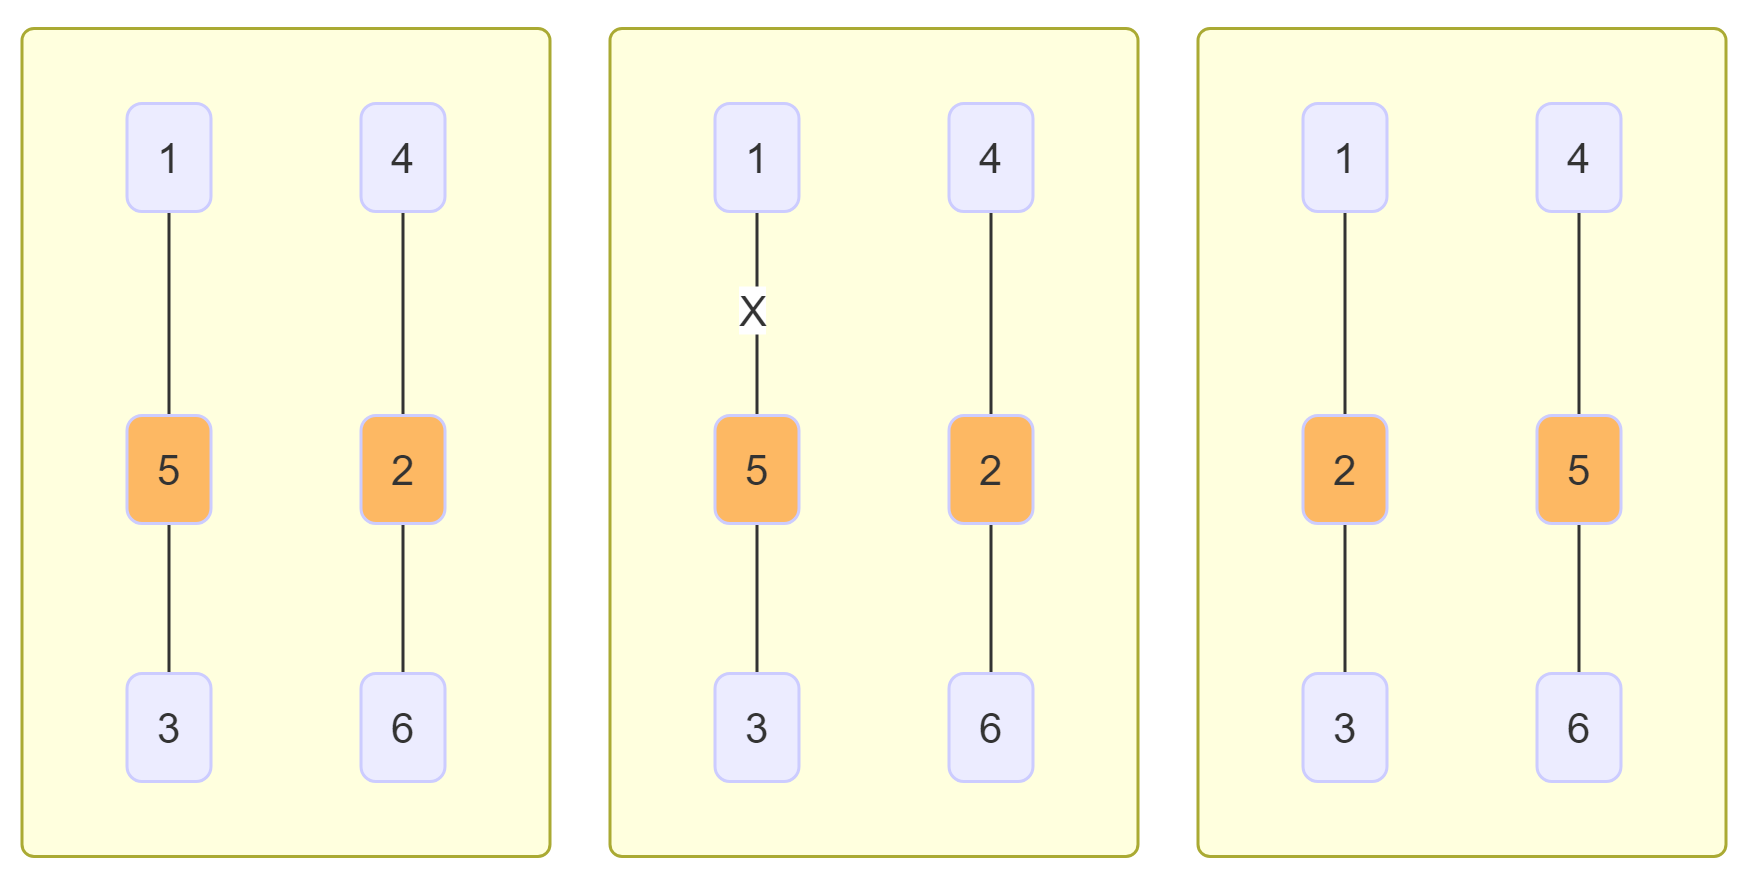
\includegraphics[width=0.75\linewidth]{degree_pre_diag} 

}

\caption{\label{fig:deg_pre} \dw{don't need explanation in main text and in the caption too - best to leave in main text. and maybe just delete the edge rather than put x through it to show it is gone} An example graph configuration that might necessitate a degree preserving swap. \textbf{Left} and \textbf{right}: two configurations of graphs whose vertices have the same degree,    \dw{fix formatting} extbf{middle}: a potential intermediary proposal. With one-step edge adding and deleting the likelihood of switching between these two graph is low if the migration rate is high enough. The degree preserving swap operator would attempt to switch between these two graphs in 1 step. Deleting the edge between city 5 and 1 (middle figure) would occur with low probability. With a migration rate of 1, this would lower city 5's count by approximately 1/3 from the true value and by half for city 1.}\label{fig:unnamed-chunk-2}
\end{figure}

\hypertarget{rewire}{%
\subsection{\texorpdfstring{\texttt{rewire()}}{rewire()}}\label{rewire}}

Rewire randomly selects an edge (v1, v2) and deletes it from the
adjacency list. It then randomly samples a vertex v3 and forms the edge
(v2, v3). Since the reverse move is selecting the edge (v2, v3) and then
rewiring (v1, v2), the Hastings ratio is 1.

\hypertarget{resultsdiscussion}{%
\section{Results/Discussion}\label{resultsdiscussion}}

\hypertarget{two-component-model}{%
\subsection{Two-Component Model}\label{two-component-model}}

\hypertarget{prior-checks-1}{%
\subsubsection{Prior Checks}\label{prior-checks-1}}

I performed prior checks where the likelihood ratio is set to 1 so that
the posterior distributions should match their prior distributions.

\begin{figure}
\centering
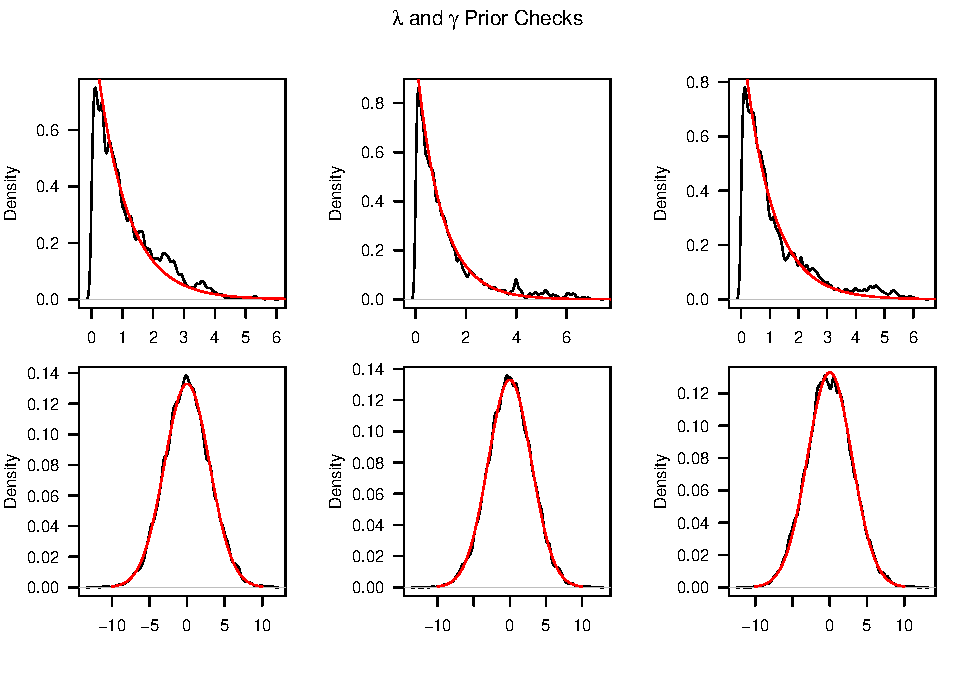
\includegraphics{thesis_draft_files/figure-latex/prior_checks_2c-1.pdf}
\caption{\label{fig:pc2c} \dw{label x axes. Also K not here.} Prior Checks for \(\gamma\), \(\lambda\) and
\(K\). Only 3 \(\lambda\) values are displayed. The KDE smoothed
distribution of values are plotted against the true density values of
the priors (that is \(P(\lambda) \sim ext{Gamma}(1,1)\) and
\(P(\gamma) \sim \text{Norm}(0,3)\). The differences appear to be
artifacts of the smoothing procedure.}
\end{figure}

The following data was collected by running 100,000 iterations (thinned
to 10,000 samples) of proposing to update either the \(\lambda\) vector,
\(\gamma\) vector, adding a change point (\(K \rightarrow K + 1\)) or
removing a change point (\(K \rightarrow K - 1\)). The likelihood ratio
was set to 1 so the only factor in accepting or rejecting a state was
the priors. As such we would expect to see the posterior distributions
of each parameter to be their respective prior distributions. The priors
are \[\vec\lambda \sim \text{Gamma}(1,1)\]
\[\vec\gamma \sim \text{Norm}(0,3)\] \[K \sim \text{Unif}(0,N)\]

In Figure \ref{fig:pc2c} we have plots of the samples of the \(\lambda\)
values (first 3) and the \(\gamma\) values. Each is overlayed with the
density of their respective priors in red. Overall there appears to be a
good match between the sampled values and their prior distributions.

In figure \ref{fig:pois_hist} we have a frequency histogram of the
sampled values of \(K\) (the number of change points) overlayed with a
red circle. The red circle represents the appropriate density value from
the prior distribution of \(K\). Overall we see a good qualitative fit
between the values sampled from the posterior and the prior
distribution. The following table gives the sample frequency and the
actual probability (from the prior distibution). If these probabilities
did not match, then there is likely a bug in the code or some unknown
prior assumption on the model. Note that the sample frequency was
computed from a thinned sample of 10,000 hence why 11, 25, and 51 have
sample probabilities of 0.0001, there was 1 occurence of each.

\begin{figure}
\centering
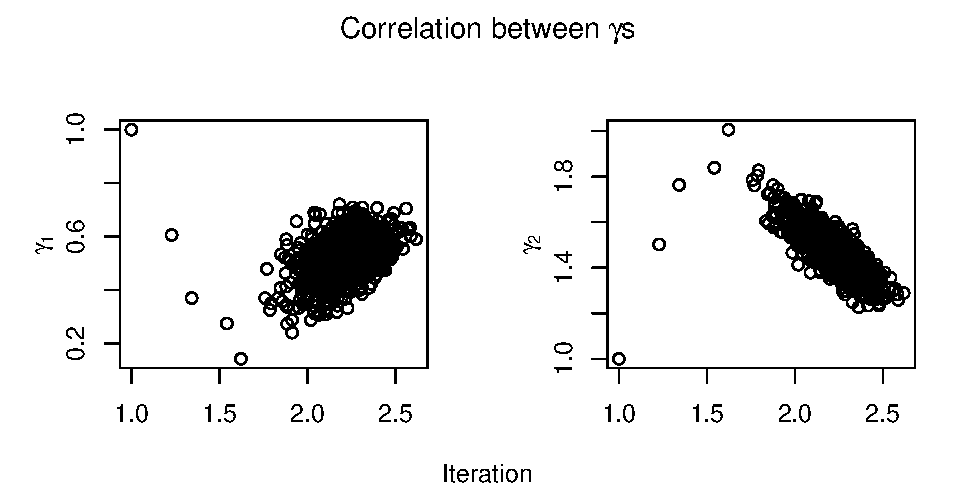
\includegraphics{thesis_draft_files/figure-latex/unnamed-chunk-3-1.pdf}
\caption{\label{fig:pois_hist} Sample probabilities of \(K\) overlayed
with true probabilities. Overall this shows a good agreement between the
sample probabilities and the true probabilties.}
\end{figure}

\dw{table unnecessary as figure is just fine}
\begin{longtable}[]{@{}ccc@{}}
\toprule
K & sample & actual\tabularnewline
\midrule
\endhead
0 & 0.136 & 0.135\tabularnewline
1 & 0.270 & 0.270\tabularnewline
2 & 0.2681 & 0.271\tabularnewline
3 & 0.185 & 0.180\tabularnewline
4 & 0.0899 & 0.902\tabularnewline
5 & 0.0365 & 0.361\tabularnewline
6 & 0.0113 & 0.012\tabularnewline
7 & 0.0029 & 0.0034\tabularnewline
8 & 0.0007 & 0.0008\tabularnewline
9 & 0.0001 & 0.00019\tabularnewline
11 & 0.0001 & 6.94e-6\tabularnewline
25 & 0.0001 & 2.97e-19\tabularnewline
51 & 0.0001 & 1.96e-52\tabularnewline
\bottomrule
\end{longtable}

\hypertarget{inference-on-simulated-data}{%
\subsubsection{Inference on Simulated
Data}\label{inference-on-simulated-data}}

\begin{longtable}[]{@{}cc@{}}
\toprule
parameters & simulation values\tabularnewline
\midrule
\endhead
K: number of changespoints & 2\tabularnewline
\(\boldsymbol{\lambda}\): epidemic parameters & 0.7, 1.2,
0.7\tabularnewline
\(\boldsymbol{\gamma}\): endemic parameters & log(10), 0.5,
1.5\tabularnewline
\(\boldsymbol{\theta}\): change points & 39, 49\tabularnewline
\bottomrule
\end{longtable}

The simulation parameters are taken from Held et al.
(\protect\hyperlink{ref-held_two-component_2006}{2006})

\begin{figure}
\centering
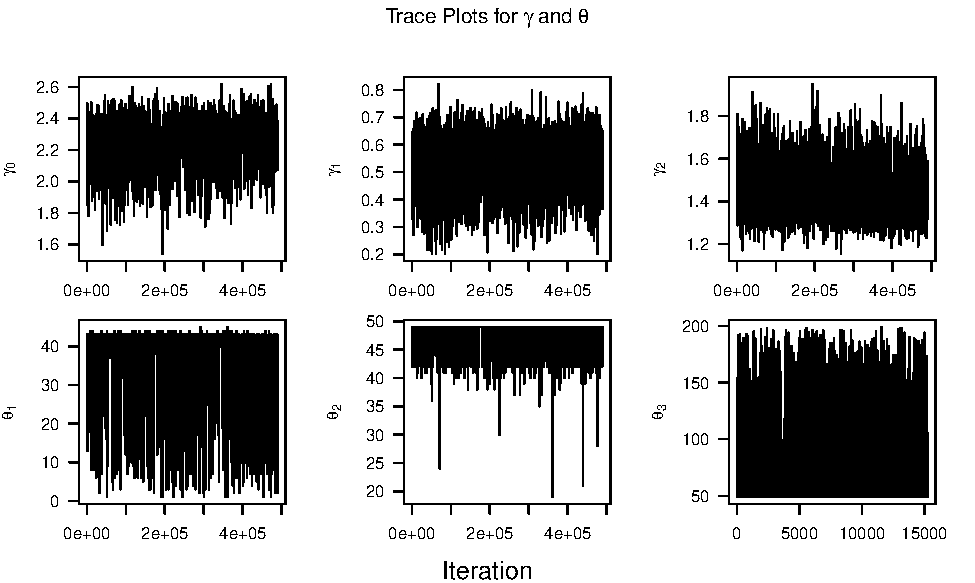
\includegraphics{thesis_draft_files/figure-latex/lambda_traces_plot-1.pdf}
\caption{\label{fig:lam_trace} Trace plots for \(\boldsymbol{\gamma}\)
and \(\boldsymbol{\theta}\). The trace plots seem relatively well mixed.
The autocorrelation is likely a function of the correlation between the
each set of \(\boldsymbol{\gamma}\) and \(\boldsymbol{\theta}\)
respectively. Thinning could potentially reduce the autocorrelation
between sample draws.}
\end{figure}

\dw{detailed comments stop here} Figure \ref{fig:lam_trace} are trace plots, which are time series of the
parameter draws. Typically a ``good'' trace plot shows no obvious
autocorrelation (which can indicate a proposal step that is too small)
or flat portions (proposal steps that are too large). Trace plots with
these patterns indicate that the sampler has not converged to the
posterior distribution of the parameter. ``Tuning'' or adjusting the
proposal jump size can help fix these patterns, with the end goal of
being able to efficiently explore the posterior distribution of the
parameter (Gelman et al.
\protect\hyperlink{ref-gelman_bayesian_2013}{2013},p. 296). The trace
plots for the \(\gamma\) parameters seem to rather well mixed though
there is a slight pattern to the \(\gamma_0\) trace plot.

\begin{figure}
\centering
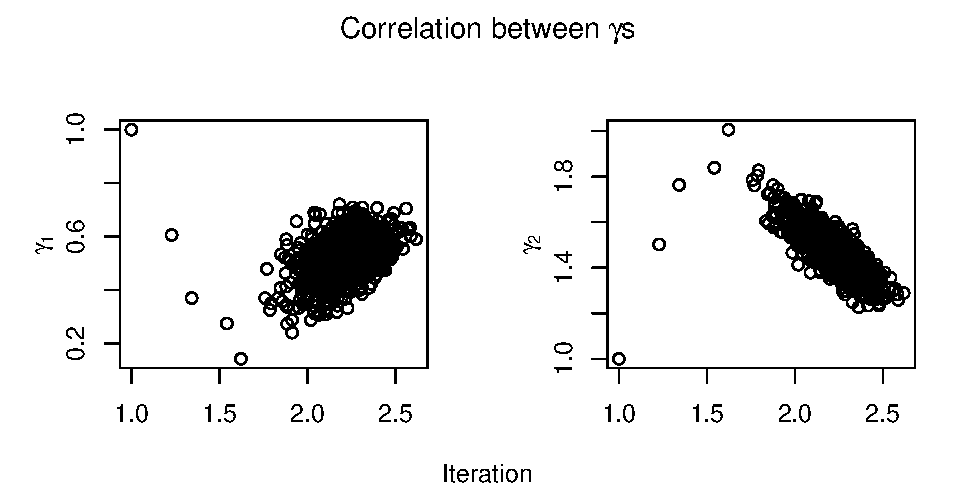
\includegraphics{thesis_draft_files/figure-latex/unnamed-chunk-4-1.pdf}
\caption{\label{fig:cor_gammas}Plots of \(\gamma_0\) vs \(\gamma_1\) and
\(\gamma_0\) vs \(\gamma_2\). Each point represents the corresponding
parameter value at the same sample draw, i.e., the values of each
parameter when the sample was accepted. The strong correlation between
the parameters can lead to poor mixing. Note the tails are due to the
initial values of the MCMC chain.}
\end{figure}

This is likely due to the correlation (see Figure \ref{fig:cor_gammas})
between \(\gamma_0\), \(\gamma_1\) and \(\gamma_2\) due to their nature
of parameterizing a cyclical function. The same is true for the
\(\theta\) parameters; they are constrained such that
\(\theta_1 < \theta_2 < \theta_3\). The dependence can cause inefficient
sampling by proposing moves that are outside these narrow
regions/combinations of parameter values (Turner et al.
\protect\hyperlink{ref-turner_method_2013}{2013}). This autocorrelation
seen in the trace plots could possibly be reduced via thinning
i.e.~taking every \(k\) samples instead of every sample. Gelman et al.
(\protect\hyperlink{ref-gelman_bayesian_2013}{2013}) mentions that they
have found it useful to store no more than a total of \(1000\)
iterations.

The \(\theta_3\) trace plot is of note because it is only valid for when
\(K = 3\); the \(\theta_3\) does not exist otherwise.\textbackslash{}

\begin{figure}

{\centering 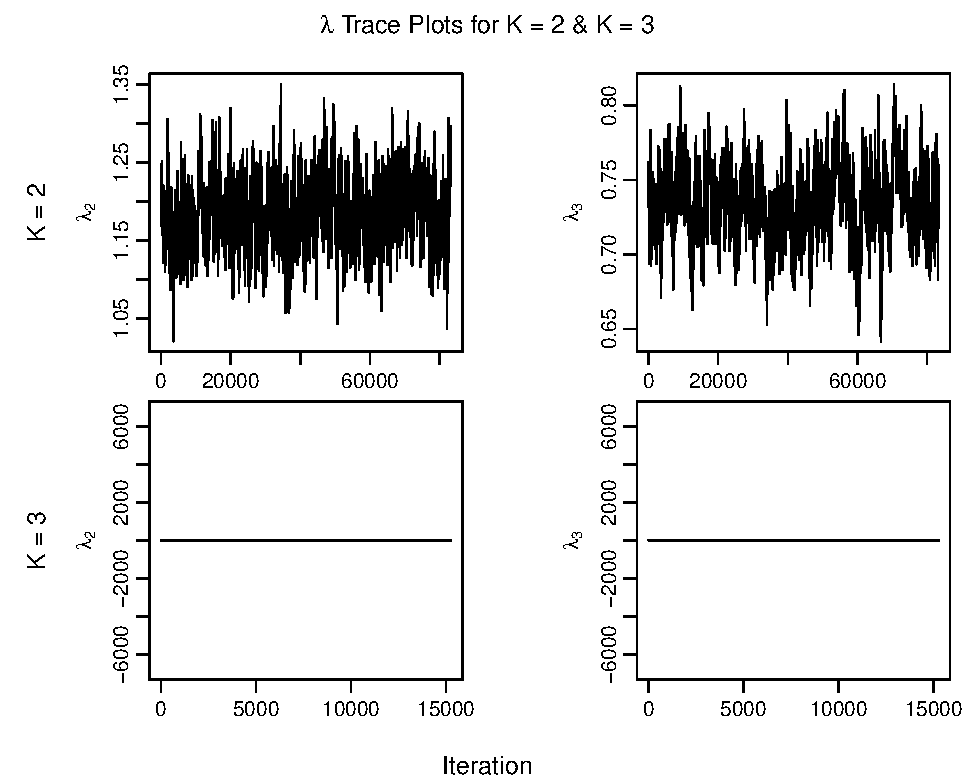
\includegraphics[height=0.41\textheight]{thesis_draft_files/figure-latex/unnamed-chunk-5-1} 

}

\caption{Trace plots for all $\lambda$ values. Overall the trace plots show that the samplers are mixing well with some minor autocorrelation that could potentially be resolved with thinning or more samples. The raw trace plots include the $\lambda$ values when there are 3 and 4 separate $\lambda$'s and is the cause of the random jumps.}\label{fig:unnamed-chunk-5}
\end{figure}

The \(\boldsymbol{\lambda}\) trace plots show that the \(\lambda_2\) and
\(\lambda_3\) traces appear to jump tightly around \(1.2\) and \(0.7\)
respectively while also jumping to \(0.7\) and \(1.2\) respectively.
This is an artifact of the dimension change in the model. When
\(K = 2\), \(\lambda_2\) is tightly fixed around \(1.2\) and
\(\lambda_3\) at \(0.7\) but when \(K = 2\), \(\lambda_3\) can take the
role of fitting the outbreak while \(\lambda_4\) models to the return
\(0.7\), the baseline.

\begin{figure}

{\centering 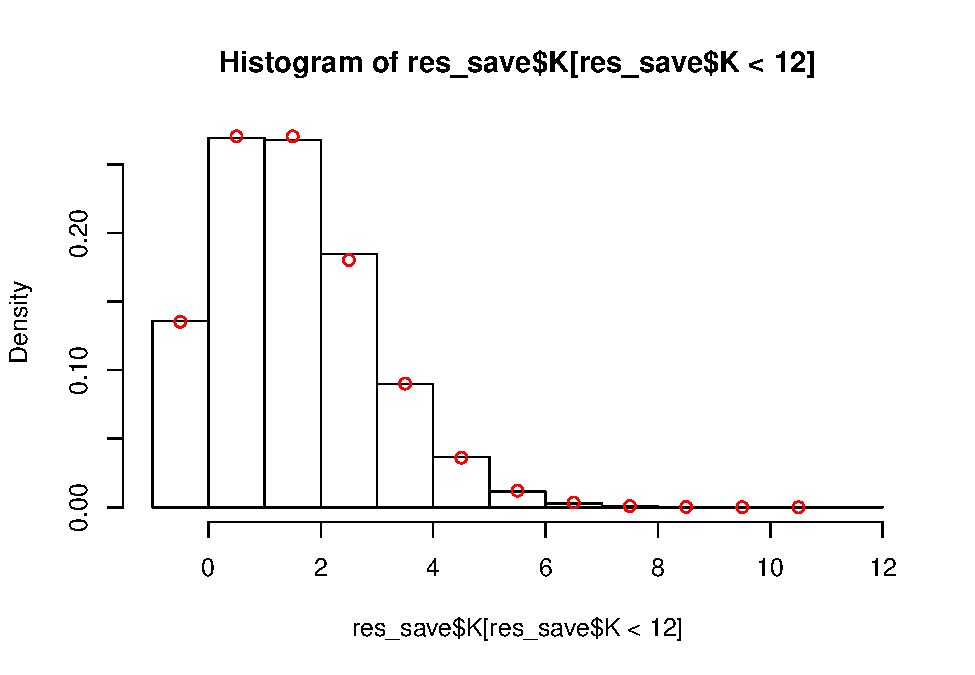
\includegraphics[height=0.41\textheight]{thesis_draft_files/figure-latex/unnamed-chunk-6-1} 

}

\caption{Trace plots filtered for K = 2 and K = 3 showing how the different number of change points affects the traces of the individual $\lambda$ values.}\label{fig:unnamed-chunk-6}
\end{figure}

\begin{figure}
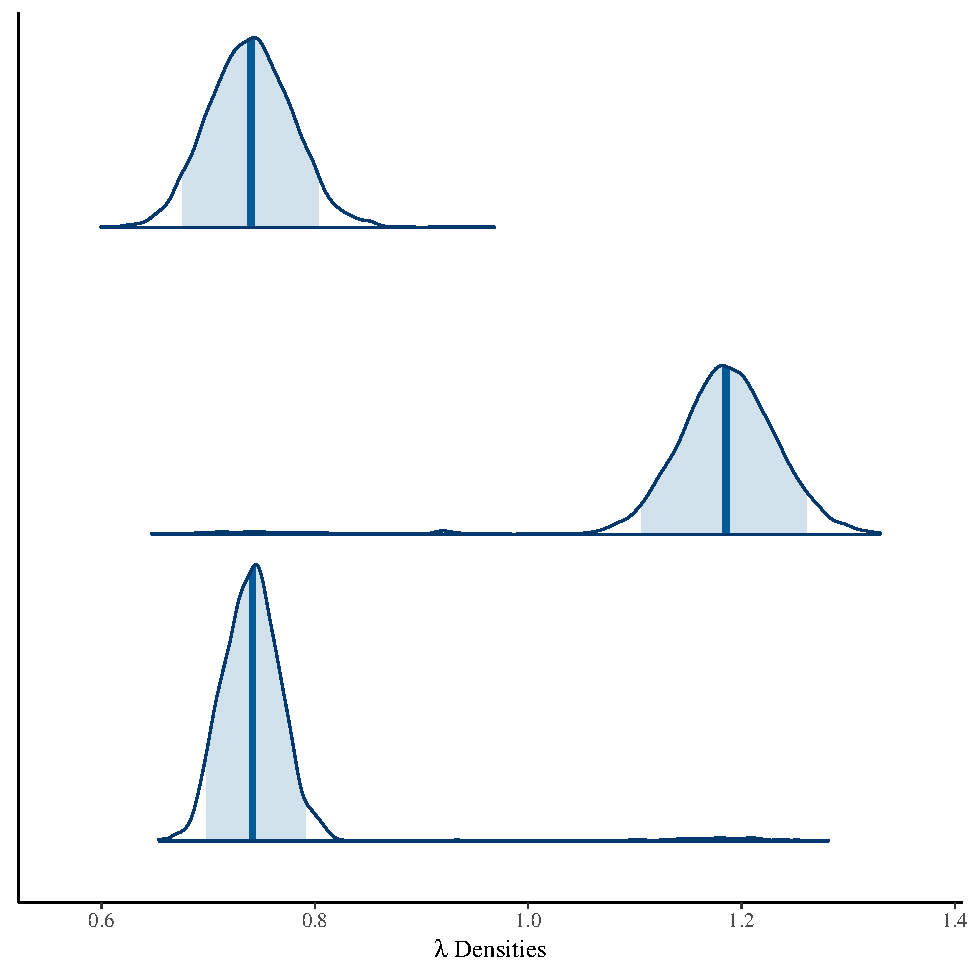
\includegraphics[width=0.47\linewidth]{thesis_draft_files/figure-latex/unnamed-chunk-7-1} 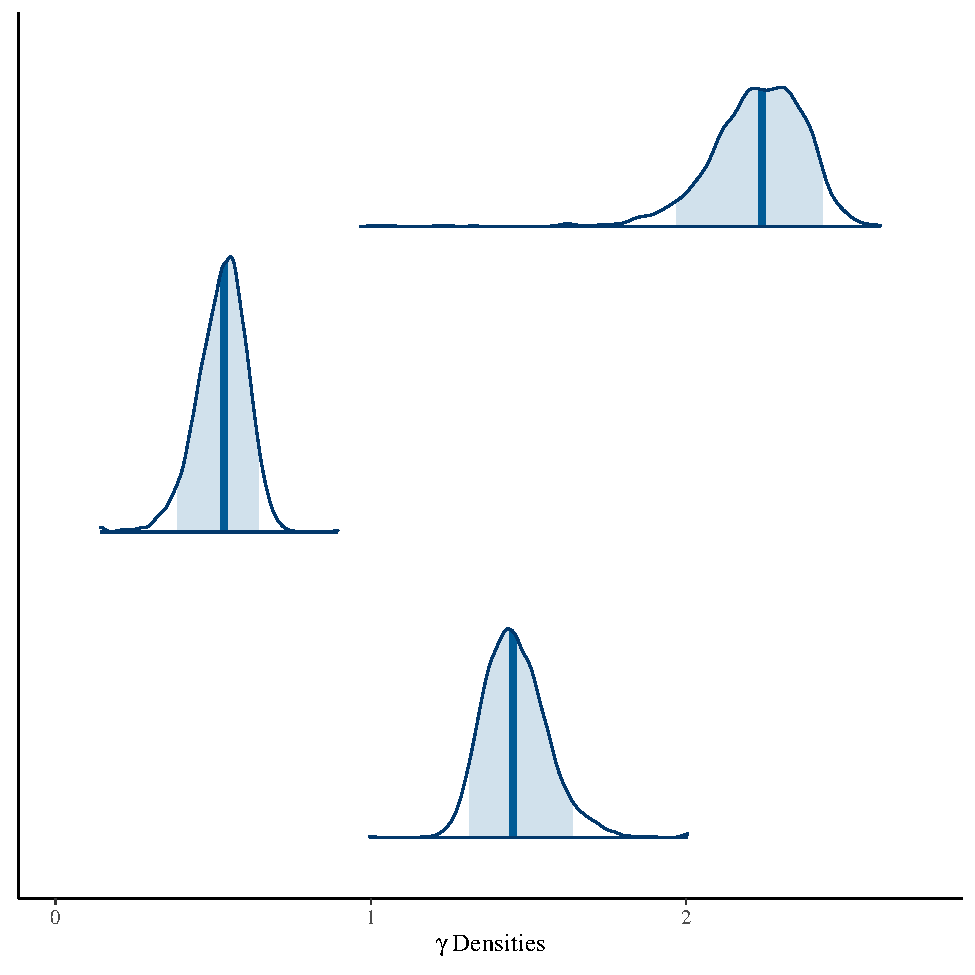
\includegraphics[width=0.47\linewidth]{thesis_draft_files/figure-latex/unnamed-chunk-7-2} \caption{\label{fig:2c_dens}\textbf{Left:} Density plots of the posterior samples of $\lambda$ parameters. The shaded blue represents the region corresponding to the 90\% highest probability density interval (HPDI). \textbf{Right:} Density plots of the posterior samples of $\gamma$ parameters. \dw{these are ugly and weirdly laid out. just use histograms. assume the long tails are there because you haven't removed burn-in?}}\label{fig:unnamed-chunk-7} 
\end{figure}

Figure \ref{fig:2c_dens}) shows the kernal density plots of the
\(\lambda\) and \(\gamma\) samples along with the area corresponding to
the 90\% highest probability density intervals (HPDIs). The 90\% HPDI is
the smallest interval that contains 90\% of the density. All HPDIs cover
their true values suggesting overall good inference.

\hypertarget{graph-estimation-on-fixed-two-component-model}{%
\subsection{Graph Estimation on Fixed Two-Component
Model}\label{graph-estimation-on-fixed-two-component-model}}

Progress on the graph. The graph proposals are a challenge to the
computational speed and mixing becomes a problem. For example the
original base graph operator was \texttt{flip\_edge()} which had much
poorer mixing than the \texttt{add/del\_edge\_op()} combination. To test
the correctness of the operators, we also set the likelihood to always
equal to 1. With the correct derivation about the priors, any
significant deviation of the posterior distributions from the prior
distributions is likely to be due to implementation errors in the code.

\hypertarget{posterior-distribution-of-number-of-edges-matches-prior-distribution}{%
\subsubsection{Posterior distribution of number of edges matches prior
distribution}\label{posterior-distribution-of-number-of-edges-matches-prior-distribution}}

Here we set the prior ratio and the likelihood ratio to always equal to
1. This places a uniform prior distribution on \(p\) and a uniform prior
on \(G|p\). Then the probability of each graph is equally likely and the
posterior distribution of the number of edges should be
\(\text{Binom}(105, 0.5)\). Figure \ref{fig:binom_hist} shows a thinned
posterior sample of the number of edges overlayed with the appropriate
\(\text{Binom}(105, 0.5)\) probabilites in red.

\begin{figure}
\centering
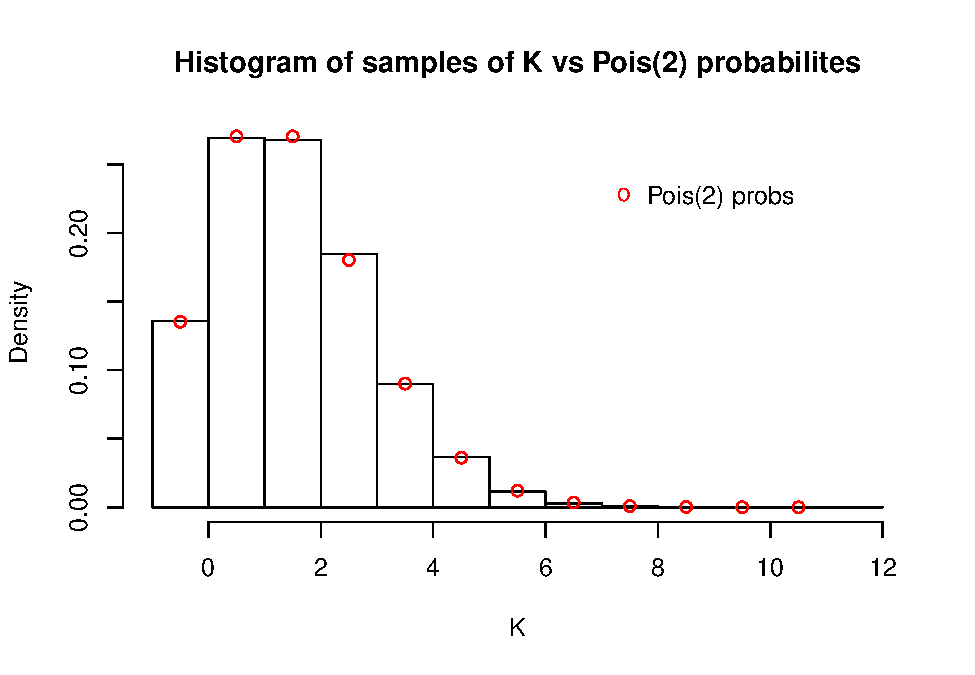
\includegraphics{thesis_draft_files/figure-latex/unnamed-chunk-8-1.pdf}
\caption{\label{fig:binom_hist} Posterior probabilities of the number of
edge counts, overlayed with true probabilities. Overall this shows a
good agreement between the posterior probabilities and the true
probabilties.}
\end{figure}

\hypertarget{inference-on-number-of-edgesp-and-migration-rate}{%
\subsubsection{\texorpdfstring{Inference on number of edges/\(p\) and
migration
rate}{Inference on number of edges/p and migration rate}}\label{inference-on-number-of-edgesp-and-migration-rate}}

\begin{longtable}[]{@{}cc@{}}
\toprule
parameters & simulation values\tabularnewline
\midrule
\endhead
K: number of changespoints & 2\tabularnewline
\(\boldsymbol{\lambda}\): epidemic parameters & 0.7, 1.2,
0.7\tabularnewline
\(\boldsymbol{\gamma}\): endemic parameters & log(10), 0.5,
1.5\tabularnewline
\(\boldsymbol{\theta}\): change points & 39, 49\tabularnewline
\(p\): Erdos-Renyi parameter & 0.15\tabularnewline
true number of edges & 12\tabularnewline
\(N_v\): number of vertices & 15\tabularnewline
\(m\): migration rate & 0.15\tabularnewline
\bottomrule
\end{longtable}

Inference is carried out on the graph and the migration rate, while the
other parameters are fixed to their true values. A single interation of
the sampler proposes adding or removing an edge (with equal probability)
25 times before proposing a migration rate change. This allows the
sampler to better explore the highly correlated posterior distribution
which can be seen in Figure \ref{fig:p_mig_pairs}.

\begin{figure}
\centering
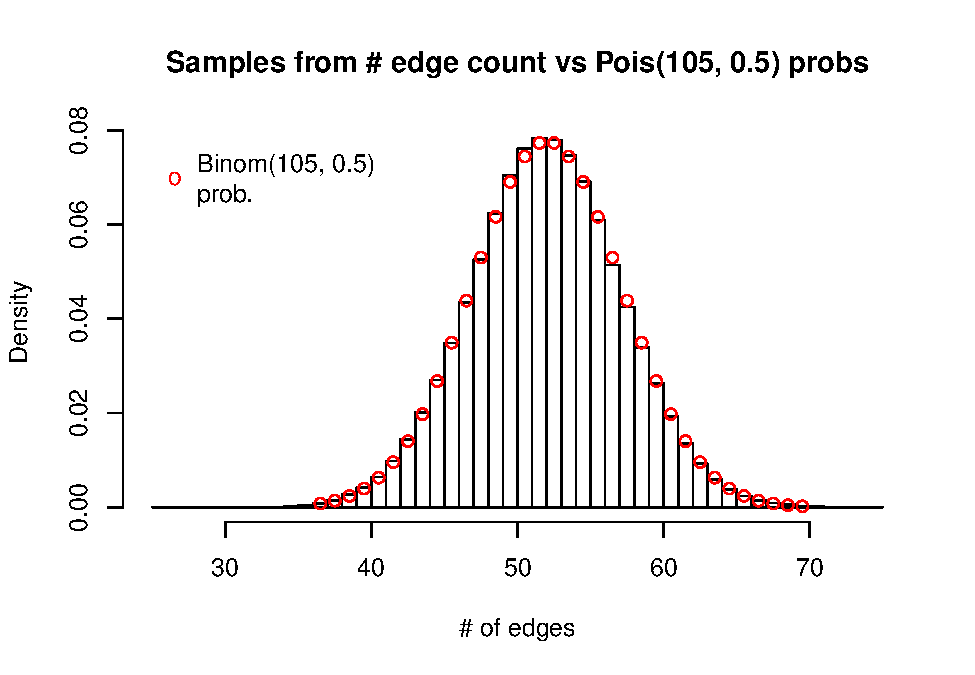
\includegraphics{thesis_draft_files/figure-latex/unnamed-chunk-9-1.pdf}
\caption{\label{fig:hist_edges} Histogram of posterior samples of the
number of edges in the graph}
\end{figure}

\hypertarget{trace-plots}{%
\subsubsection{trace plots}\label{trace-plots}}

\dw{turn this figure into a float. It should not great mixing -- you need to run it longer}
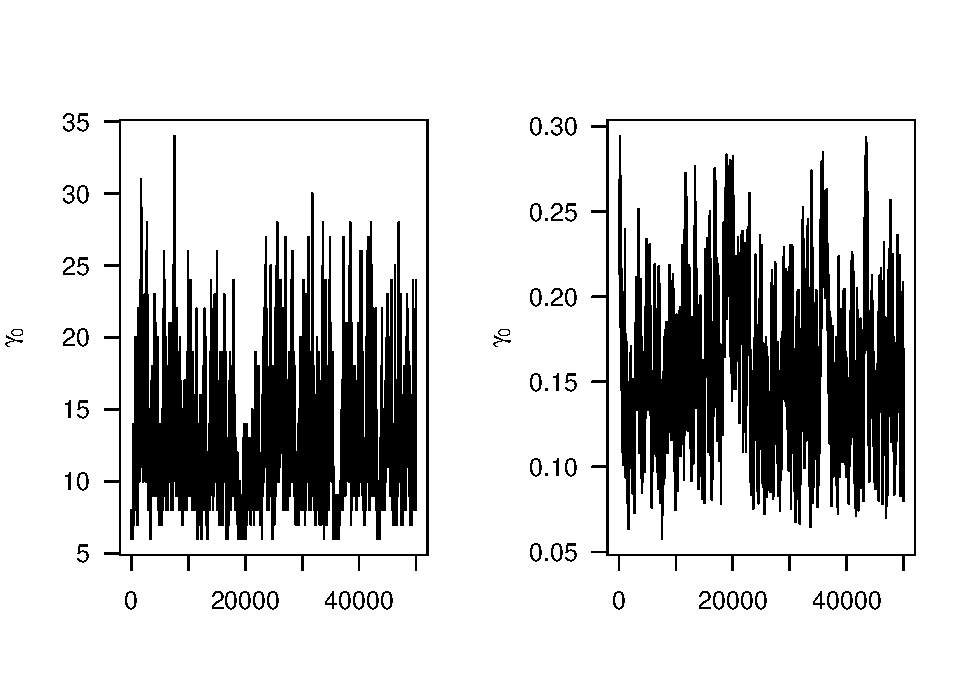
\includegraphics{thesis_draft_files/figure-latex/unnamed-chunk-10-1.pdf}

Figure \ref{fig:hist_edges} is a histogram of the posterior samples of
the number of edges in the graph. The mean of the distribution is
12.41644 and median is 12 and the mode is numeric. The mean and median
are close to the true number of edges in the graph, \(12\).

Figure \ref{fig:p_mig_pairs} also shows on the left, a hex plot of the
joint posterior samples of \(p\) (which is computed by 15/105 where 105
is the maximum number of edges in a graph with 15 vertices ) and
migration rate. It shows a strong negative correlation, which is to
expected. If the migration rate is smaller than the true value \(m\),
say \(0.5m\) then the a city connected to \(d\) cities would need to
connect to \(2d\) to have the ``correct'' counts. Similarly the
migration rate is higher than the true migration, then the number of
edges would need to be lower than the true number of edges. tk need to
explain this

Figure \ref{fig:p_mig_pairs} also shows the kernal density estimates of
\(p\) and migration rate. Both of the 90\% HPDIs cover their true
values.

\begin{figure}
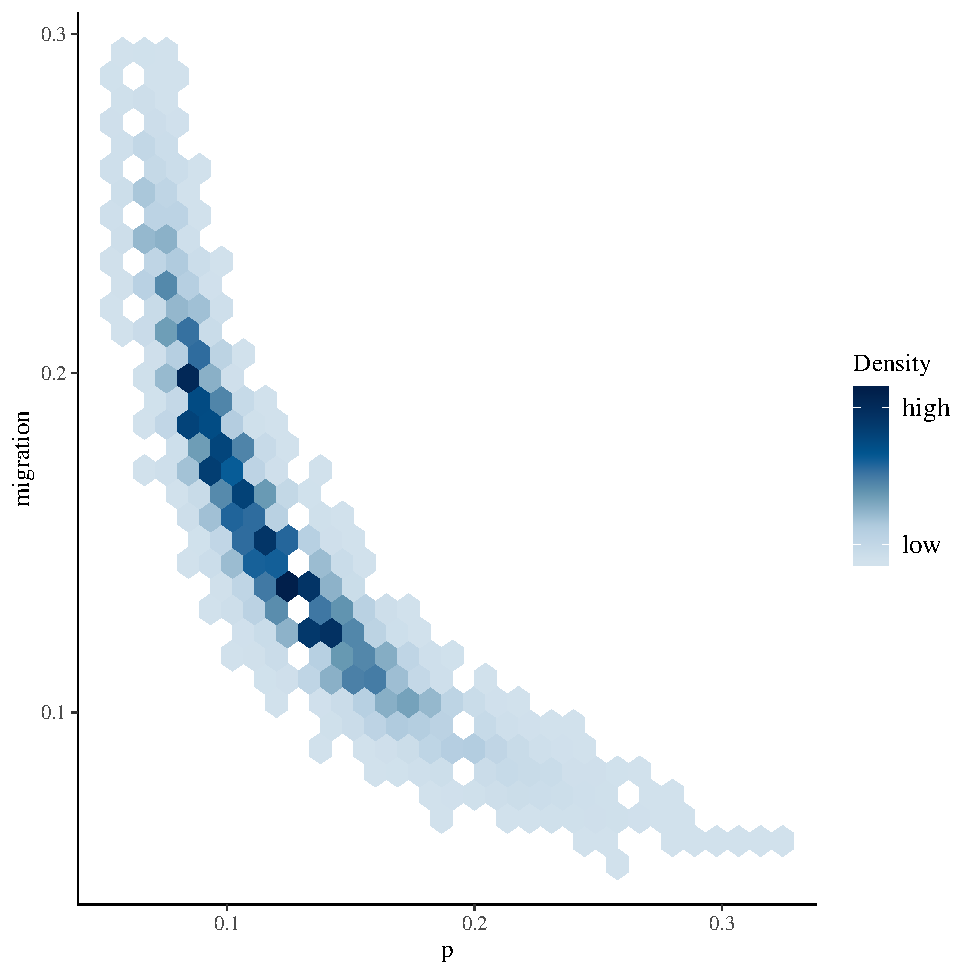
\includegraphics[width=0.5\linewidth]{thesis_draft_files/figure-latex/unnamed-chunk-11-1} 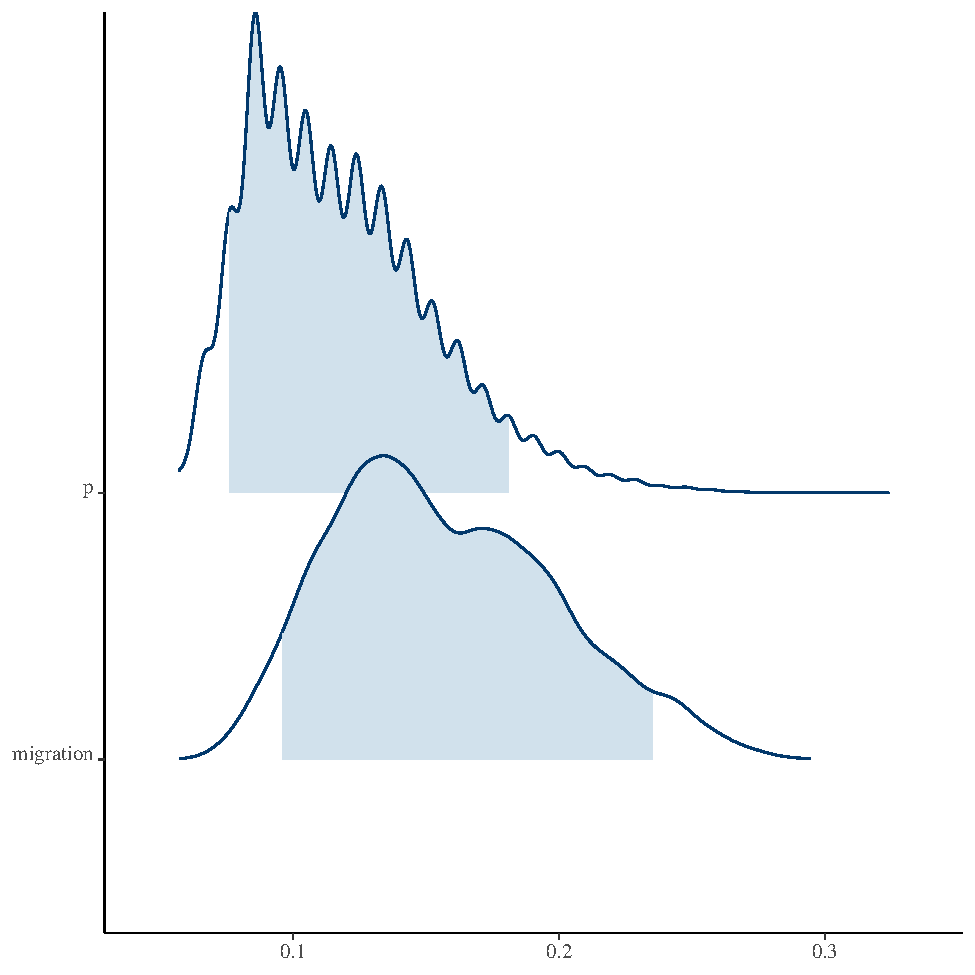
\includegraphics[width=0.5\linewidth]{thesis_draft_files/figure-latex/unnamed-chunk-11-2} \caption{\label{fig:p_mig_pairs} \textbf{Left:} Joint posterior hex plot between migration rate and $p$ the parameter for the Erdos-Renyi graph. The $p$ value is directly computed from the number of edges by dividing by the total possible edges which is 105. The plot shows a strong negative correlation between $p$ and the migration rate.  \textbf{Right:} Density plots with regions corresponding to the 90\% highest density probability intervals in blue. }\label{fig:unnamed-chunk-11}
\end{figure}

\hypertarget{traces-showing-the-parameter-space-moves}{%
\section{Traces showing the parameter space
moves}\label{traces-showing-the-parameter-space-moves}}

\dw{this is missing from repo}
%\includegraphics{thesis_draft_files/figure-latex/unnamed-chunk-12-1.pdf}

\pagebreak

\hypertarget{conclusion}{%
\section{Conclusion}\label{conclusion}}

Conclusion here

\hypertarget{future-extensions}{%
\subsubsection{Future Extensions}\label{future-extensions}}

While this thesis only covers a fixed migration rate, the end goal would
be to model the migration rate as a function of city specific
attributes, e.g.~size of the cities, distance between the cities, if the
cities are near large highways or have ports for shipping. Then \(m\)
can be modelled as a logistic function of these city parameters
\(m \sim logit(\beta_0 + \beta_1*X_1 + \beta_2*X_2 + \dots)\). This
would allow estimation of which city specific attributes cause the
highest migration.

\pagebreak

\hypertarget{extra-graphs}{%
\subsection{extra graphs}\label{extra-graphs}}

\begin{figure}
\centering
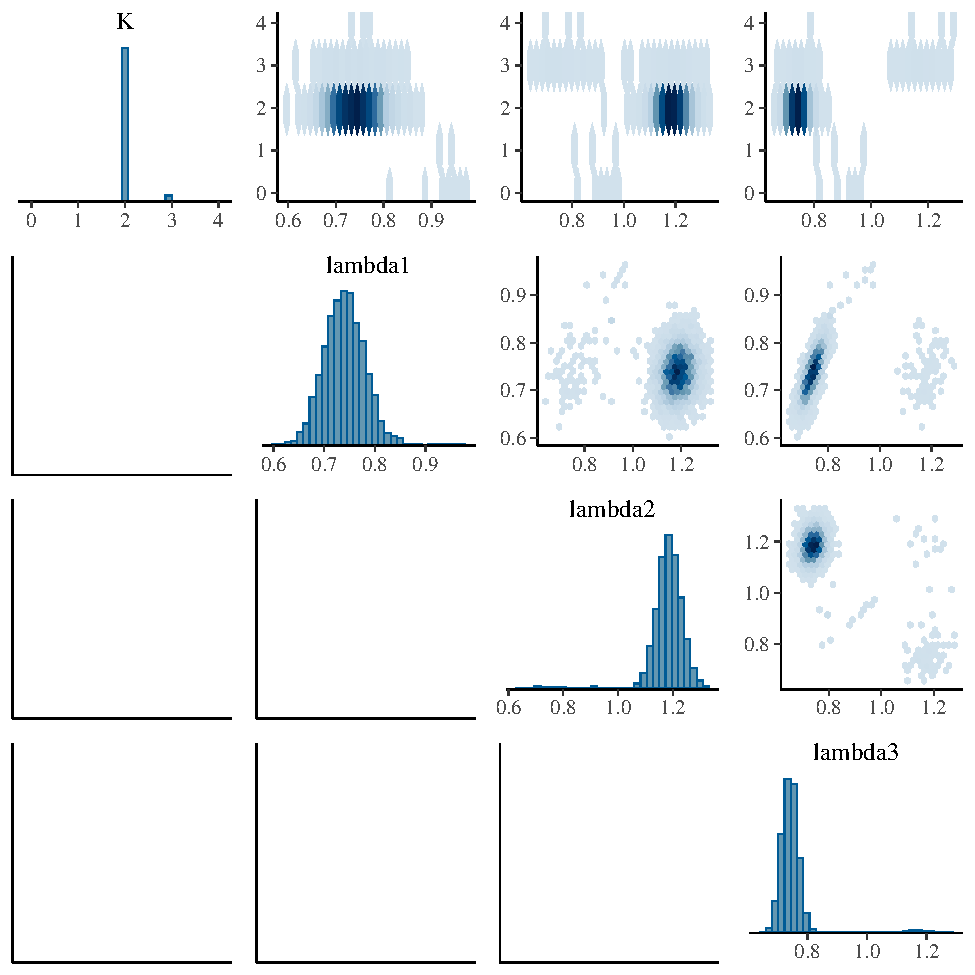
\includegraphics{thesis_draft_files/figure-latex/unnamed-chunk-13-1.pdf}
\caption{\label{fig:pairs_lambda} density plots}
\end{figure}

\begin{figure}
\centering
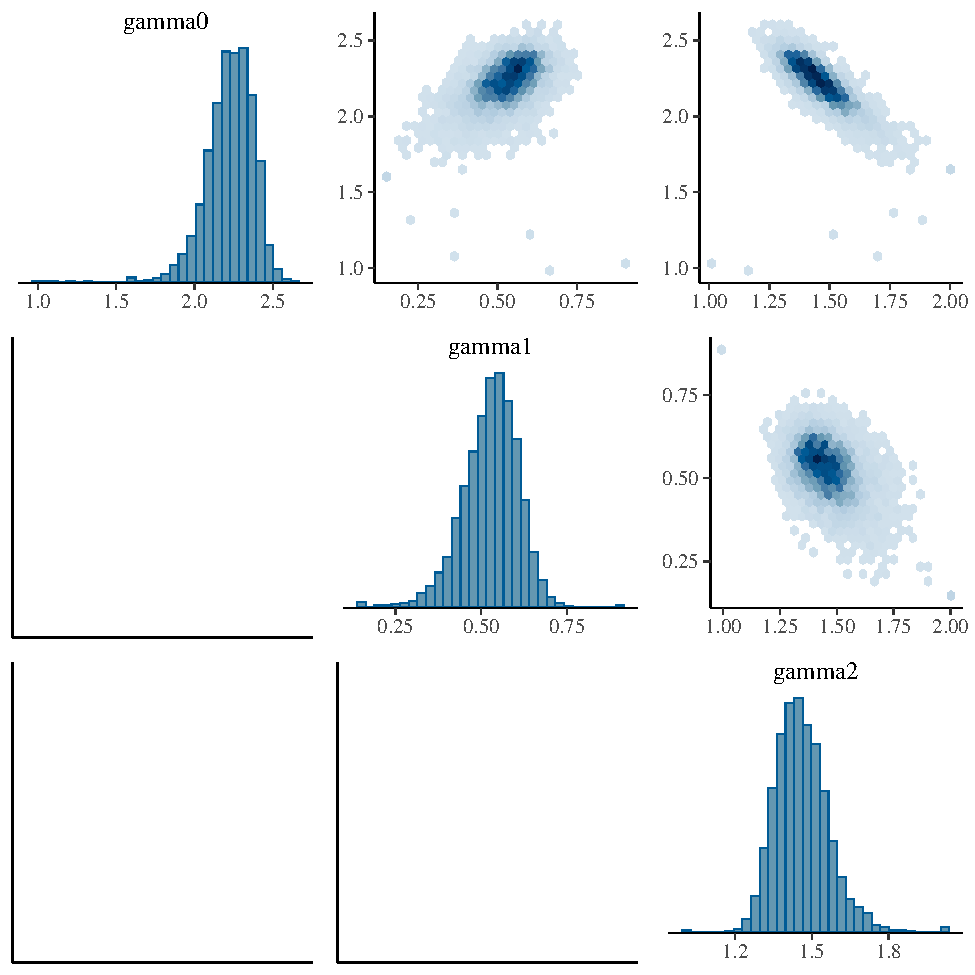
\includegraphics{thesis_draft_files/figure-latex/unnamed-chunk-14-1.pdf}
\caption{\label{fig:pairs_gamma} dens plots}
\end{figure}

\pagebreak

\hypertarget{citations}{%
\section*{Citations}\label{citations}}
\addcontentsline{toc}{section}{Citations}

\hypertarget{refs}{}
\leavevmode\hypertarget{ref-carpenter_bayesian_2017}{}%
Carpenter, B. (2017), ``Bayesian Posteriors are Calibrated by
Definition,'' \emph{Statistical Modeling, Causal Inference, and Social
Science}.

\leavevmode\hypertarget{ref-cook_validation_2006}{}%
Cook, S. R., Gelman, A., and Rubin, D. B. (2006), ``Validation of
Software for Bayesian Models Using Posterior Quantiles,'' \emph{Journal
of Computational and Graphical Statistics}, 15, 675--692.

\leavevmode\hypertarget{ref-diggle_-line_2003}{}%
Diggle, P., Knorr-Held, L., Rowlingson, B., Su, T., Hawtin, P., and
Bryant, T. (2003), ``On-line Monitoring of Public Health Surveillance
Data,'' pp. 233--266.
\url{https://doi.org/10.1093/acprof:oso/9780195146493.003.0009}.

\leavevmode\hypertarget{ref-eddelbuettel_rcpp_2011}{}%
Eddelbuettel, D., and François, R. (2011), ``Rcpp: Seamless R and C++
Integration,'' \emph{Journal of Statistical Software}, 40, 1--18.
\url{https://doi.org/10.18637/jss.v040.i08}.

\leavevmode\hypertarget{ref-noauthor_ehec_2011}{}%
\emph{EHEC O104:H4 Outbreak Germany 2011} (2011), report, Robert
Koch-Institut; Robert Koch-Institut, Infektionsepidemiologie.
\url{https://doi.org/http://dx.doi.org/10.25646/88}.

\leavevmode\hypertarget{ref-gelman_bayesian_2013}{}%
Gelman, A., Carlin, J. B., Stern, H. S., Dunson, D. B., Vehtari, A., and
Rubin, D. B. (2013), \emph{Bayesian Data Analysis, Third Edition}, CRC
Press.

\leavevmode\hypertarget{ref-green_reversible_1995}{}%
Green, P. J. (1995), ``Reversible jump Markov chain Monte Carlo
computation and Bayesian model determination.''
\url{https://doi.org/10.1093/biomet/82.4.711}.

\leavevmode\hypertarget{ref-grimmett_probability_2004}{}%
Grimmett, G., and Stirzaker, D. (2004), \emph{Probability and random
processes}, Oxford Oxford University Press.

\leavevmode\hypertarget{ref-groendyke_bayesian_2011}{}%
Groendyke, C., Welch, D., and Hunter, D. R. (2011), ``Bayesian Inference
for Contact Networks Given Epidemic Data,'' \emph{Scandinavian Journal
of Statistics}, 38, 600--616.
\url{https://doi.org/10.1111/j.1467-9469.2010.00721.x}.

\leavevmode\hypertarget{ref-held_two-component_2006}{}%
Held, L., Hofmann, M., Höhle, M., and Schmid, V. (2006), ``A
two-component model for counts of infectious diseases,''
\emph{Biostatistics}, 7, 422--437.
\url{https://doi.org/10.1093/biostatistics/kxj016}.

\leavevmode\hypertarget{ref-horner_hash_2015}{}%
Horner, J. (2015), ``Hash Table Performance in R: Part I,''
\emph{R-bloggers}.

\leavevmode\hypertarget{ref-keeling_modeling_2008}{}%
Keeling, M. J., and Rohani, P. (2008), \emph{Modeling Infectious
Diseases in Humans and Animals}, Princeton University Press.

\leavevmode\hypertarget{ref-kruschke_doing_2014}{}%
Kruschke, J. (2014), \emph{Doing Bayesian Data Analysis: A Tutorial with
R, JAGS, and Stan}, Academic Press.

\leavevmode\hypertarget{ref-pawitan_all_2001}{}%
Pawitan, Y. (2001), \emph{In All Likelihood: Statistical Modelling and
Inference Using Likelihood}, OUP Oxford.

\leavevmode\hypertarget{ref-r_core_team_r_2019}{}%
R Core Team (2019), \emph{R: A Language and Environment for Statistical
Computing}, Vienna, Austria: R Foundation for Statistical Computing.

\leavevmode\hypertarget{ref-turner_method_2013}{}%
Turner, B. M., Sederberg, P. B., Brown, S. D., and Steyvers, M. (2013),
``A Method for Efficiently Sampling From Distributions With Correlated
Dimensions,'' \emph{Psychological methods}, 18, 368--384.
\url{https://doi.org/10.1037/a0032222}.


\end{document}
